% Created by tikzDevice version 0.6.1 on 2016-05-16 21:46:23
% !TEX encoding = UTF-8 Unicode
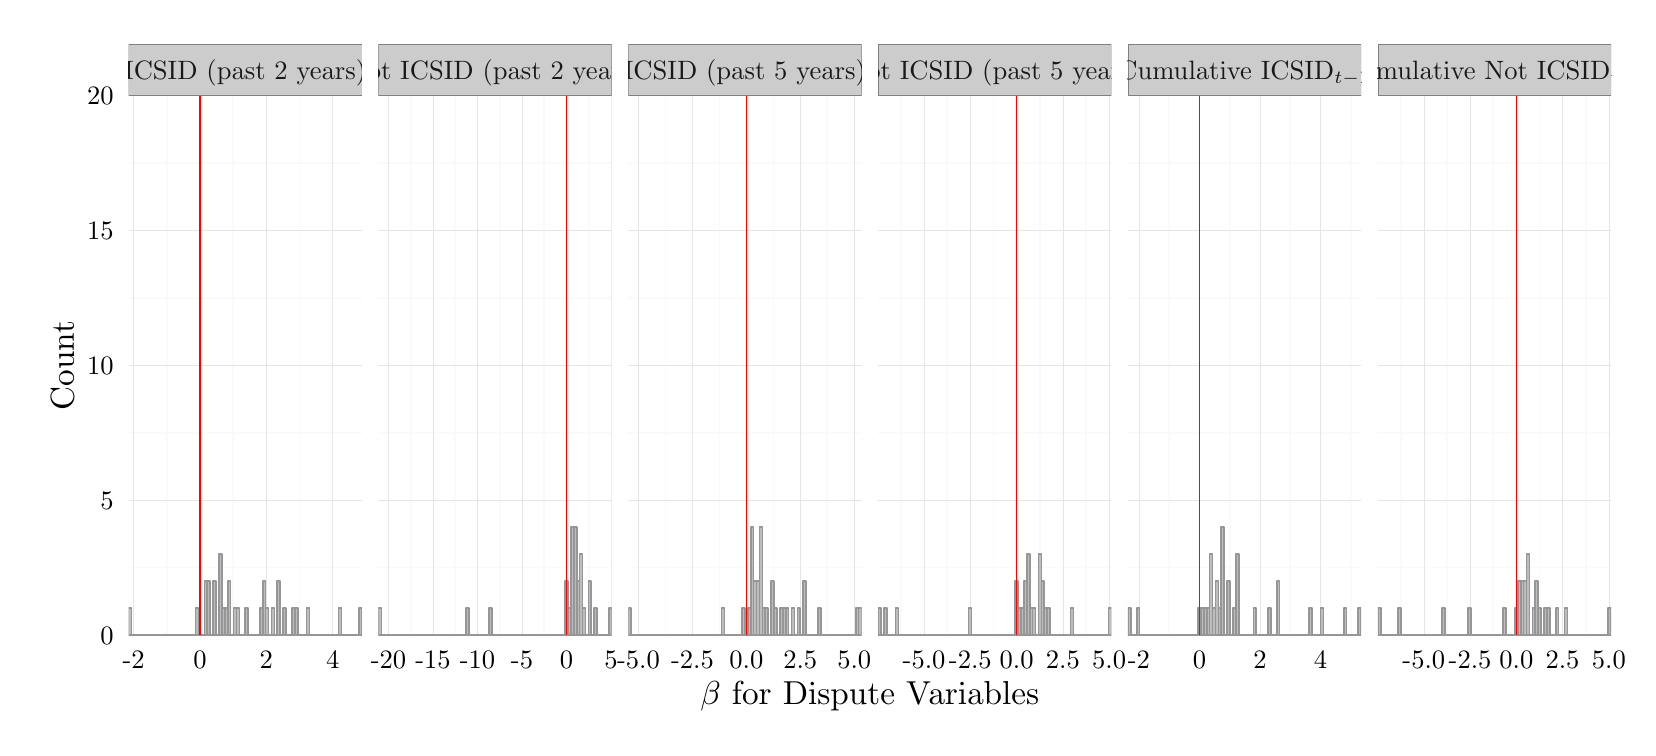
\begin{tikzpicture}[x=1pt,y=1pt]
\definecolor[named]{drawColor}{rgb}{0.00,0.00,0.00}
\definecolor[named]{fillColor}{rgb}{1.00,1.00,1.00}
\fill[color=fillColor,] (0,0) rectangle (578.16,252.94);
\begin{scope}
\path[clip] (  0.00,  0.00) rectangle (578.16,252.94);
\end{scope}
\begin{scope}
\path[clip] (  0.00,  0.00) rectangle (578.16,252.94);
\end{scope}
\begin{scope}
\path[clip] (  0.00,  0.00) rectangle (578.16,252.94);
\end{scope}
\begin{scope}
\path[clip] (  0.00,  0.00) rectangle (578.16,252.94);
\end{scope}
\begin{scope}
\path[clip] (  0.00,  0.00) rectangle (578.16,252.94);
\end{scope}
\begin{scope}
\path[clip] (  0.00,  0.00) rectangle (578.16,252.94);
\end{scope}
\begin{scope}
\path[clip] (  0.00,  0.00) rectangle (578.16,252.94);
\end{scope}
\begin{scope}
\path[clip] (  0.00,  0.00) rectangle (578.16,252.94);
\end{scope}
\begin{scope}
\path[clip] (  0.00,  0.00) rectangle (578.16,252.94);
\end{scope}
\begin{scope}
\path[clip] (  0.00,  0.00) rectangle (578.16,252.94);
\end{scope}
\begin{scope}
\path[clip] (  0.00,  0.00) rectangle (578.16,252.94);
\end{scope}
\begin{scope}
\path[clip] (  0.00,  0.00) rectangle (578.16,252.94);
\end{scope}
\begin{scope}
\path[clip] (  0.00,  0.00) rectangle (578.16,252.94);
\end{scope}
\begin{scope}
\path[clip] (  0.00,  0.00) rectangle (578.16,252.94);
\end{scope}
\begin{scope}
\path[clip] (  0.00,  0.00) rectangle (578.16,252.94);
\end{scope}
\begin{scope}
\path[clip] (  0.00,  0.00) rectangle (578.16,252.94);
\end{scope}
\begin{scope}
\path[clip] (  0.00,  0.00) rectangle (578.16,252.94);
\end{scope}
\begin{scope}
\path[clip] (  0.00,  0.00) rectangle (578.16,252.94);
\end{scope}
\begin{scope}
\path[clip] (  0.00,  0.00) rectangle (578.16,252.94);
\end{scope}
\begin{scope}
\path[clip] (  0.00,  0.00) rectangle (578.16,252.94);
\end{scope}
\begin{scope}
\path[clip] (  0.00,  0.00) rectangle (578.16,252.94);
\end{scope}
\begin{scope}
\path[clip] (  0.00,  0.00) rectangle (578.16,252.94);
\end{scope}
\begin{scope}
\path[clip] (  0.00,  0.00) rectangle (578.16,252.94);
\end{scope}
\begin{scope}
\path[clip] (  0.00,  0.00) rectangle (578.16,252.94);
\end{scope}
\begin{scope}
\path[clip] (  0.00,  0.00) rectangle (578.16,252.94);
\end{scope}
\begin{scope}
\path[clip] (  0.00,  0.00) rectangle (578.16,252.94);
\definecolor[named]{drawColor}{rgb}{1.00,1.00,1.00}
\definecolor[named]{fillColor}{rgb}{1.00,1.00,1.00}

\draw[color=drawColor,line width= 0.6pt,line cap=round,line join=round,fill=fillColor,] (  0.00,  0.00) rectangle (578.16,252.95);
\end{scope}
\begin{scope}
\path[clip] (  0.00,  0.00) rectangle (578.16,252.94);
\end{scope}
\begin{scope}
\path[clip] ( 36.46, 33.48) rectangle (120.75,228.33);
\definecolor[named]{fillColor}{rgb}{1.00,1.00,1.00}

\draw[fill=fillColor,draw opacity=0.00,] ( 36.46, 33.48) rectangle (120.75,228.33);
\definecolor[named]{drawColor}{rgb}{0.98,0.98,0.98}

\draw[color=drawColor,line width= 0.6pt,line join=round,fill opacity=0.00,] ( 36.46, 57.83) --
	(120.75, 57.83);

\draw[color=drawColor,line width= 0.6pt,line join=round,fill opacity=0.00,] ( 36.46,106.55) --
	(120.75,106.55);

\draw[color=drawColor,line width= 0.6pt,line join=round,fill opacity=0.00,] ( 36.46,155.26) --
	(120.75,155.26);

\draw[color=drawColor,line width= 0.6pt,line join=round,fill opacity=0.00,] ( 36.46,203.98) --
	(120.75,203.98);

\draw[color=drawColor,line width= 0.6pt,line join=round,fill opacity=0.00,] ( 50.28, 33.48) --
	( 50.28,228.33);

\draw[color=drawColor,line width= 0.6pt,line join=round,fill opacity=0.00,] ( 74.27, 33.48) --
	( 74.27,228.33);

\draw[color=drawColor,line width= 0.6pt,line join=round,fill opacity=0.00,] ( 98.25, 33.48) --
	( 98.25,228.33);
\definecolor[named]{drawColor}{rgb}{0.90,0.90,0.90}

\draw[color=drawColor,line width= 0.2pt,line join=round,fill opacity=0.00,] ( 36.46, 33.48) --
	(120.75, 33.48);

\draw[color=drawColor,line width= 0.2pt,line join=round,fill opacity=0.00,] ( 36.46, 82.19) --
	(120.75, 82.19);

\draw[color=drawColor,line width= 0.2pt,line join=round,fill opacity=0.00,] ( 36.46,130.90) --
	(120.75,130.90);

\draw[color=drawColor,line width= 0.2pt,line join=round,fill opacity=0.00,] ( 36.46,179.62) --
	(120.75,179.62);

\draw[color=drawColor,line width= 0.2pt,line join=round,fill opacity=0.00,] ( 36.46,228.33) --
	(120.75,228.33);

\draw[color=drawColor,line width= 0.2pt,line join=round,fill opacity=0.00,] ( 38.29, 33.48) --
	( 38.29,228.33);

\draw[color=drawColor,line width= 0.2pt,line join=round,fill opacity=0.00,] ( 62.27, 33.48) --
	( 62.27,228.33);

\draw[color=drawColor,line width= 0.2pt,line join=round,fill opacity=0.00,] ( 86.26, 33.48) --
	( 86.26,228.33);

\draw[color=drawColor,line width= 0.2pt,line join=round,fill opacity=0.00,] (110.24, 33.48) --
	(110.24,228.33);
\definecolor[named]{drawColor}{rgb}{0.59,0.59,0.59}
\definecolor[named]{fillColor}{rgb}{0.74,0.74,0.74}

\draw[color=drawColor,line width= 0.6pt,line join=round,fill=fillColor,] ( 36.46, 33.48) rectangle ( 37.52, 43.22);

\draw[color=drawColor,line width= 0.6pt,line join=round,fill=fillColor,] ( 37.52, 33.48) rectangle ( 38.57, 33.48);

\draw[color=drawColor,line width= 0.6pt,line join=round,fill=fillColor,] ( 38.57, 33.48) rectangle ( 39.62, 33.48);

\draw[color=drawColor,line width= 0.6pt,line join=round,fill=fillColor,] ( 39.62, 33.48) rectangle ( 40.68, 33.48);

\draw[color=drawColor,line width= 0.6pt,line join=round,fill=fillColor,] ( 40.68, 33.48) rectangle ( 41.73, 33.48);

\draw[color=drawColor,line width= 0.6pt,line join=round,fill=fillColor,] ( 41.73, 33.48) rectangle ( 42.78, 33.48);

\draw[color=drawColor,line width= 0.6pt,line join=round,fill=fillColor,] ( 42.78, 33.48) rectangle ( 43.84, 33.48);

\draw[color=drawColor,line width= 0.6pt,line join=round,fill=fillColor,] ( 43.84, 33.48) rectangle ( 44.89, 33.48);

\draw[color=drawColor,line width= 0.6pt,line join=round,fill=fillColor,] ( 44.89, 33.48) rectangle ( 45.94, 33.48);

\draw[color=drawColor,line width= 0.6pt,line join=round,fill=fillColor,] ( 45.94, 33.48) rectangle ( 47.00, 33.48);

\draw[color=drawColor,line width= 0.6pt,line join=round,fill=fillColor,] ( 47.00, 33.48) rectangle ( 48.05, 33.48);

\draw[color=drawColor,line width= 0.6pt,line join=round,fill=fillColor,] ( 48.05, 33.48) rectangle ( 49.10, 33.48);

\draw[color=drawColor,line width= 0.6pt,line join=round,fill=fillColor,] ( 49.10, 33.48) rectangle ( 50.16, 33.48);

\draw[color=drawColor,line width= 0.6pt,line join=round,fill=fillColor,] ( 50.16, 33.48) rectangle ( 51.21, 33.48);

\draw[color=drawColor,line width= 0.6pt,line join=round,fill=fillColor,] ( 51.21, 33.48) rectangle ( 52.27, 33.48);

\draw[color=drawColor,line width= 0.6pt,line join=round,fill=fillColor,] ( 52.27, 33.48) rectangle ( 53.32, 33.48);

\draw[color=drawColor,line width= 0.6pt,line join=round,fill=fillColor,] ( 53.32, 33.48) rectangle ( 54.37, 33.48);

\draw[color=drawColor,line width= 0.6pt,line join=round,fill=fillColor,] ( 54.37, 33.48) rectangle ( 55.43, 33.48);

\draw[color=drawColor,line width= 0.6pt,line join=round,fill=fillColor,] ( 55.43, 33.48) rectangle ( 56.48, 33.48);

\draw[color=drawColor,line width= 0.6pt,line join=round,fill=fillColor,] ( 56.48, 33.48) rectangle ( 57.53, 33.48);

\draw[color=drawColor,line width= 0.6pt,line join=round,fill=fillColor,] ( 57.53, 33.48) rectangle ( 58.59, 33.48);

\draw[color=drawColor,line width= 0.6pt,line join=round,fill=fillColor,] ( 58.59, 33.48) rectangle ( 59.64, 33.48);

\draw[color=drawColor,line width= 0.6pt,line join=round,fill=fillColor,] ( 59.64, 33.48) rectangle ( 60.69, 33.48);

\draw[color=drawColor,line width= 0.6pt,line join=round,fill=fillColor,] ( 60.69, 33.48) rectangle ( 61.75, 43.22);

\draw[color=drawColor,line width= 0.6pt,line join=round,fill=fillColor,] ( 61.75, 33.48) rectangle ( 62.80, 33.48);

\draw[color=drawColor,line width= 0.6pt,line join=round,fill=fillColor,] ( 62.80, 33.48) rectangle ( 63.85, 33.48);

\draw[color=drawColor,line width= 0.6pt,line join=round,fill=fillColor,] ( 63.85, 33.48) rectangle ( 64.91, 52.96);

\draw[color=drawColor,line width= 0.6pt,line join=round,fill=fillColor,] ( 64.91, 33.48) rectangle ( 65.96, 52.96);

\draw[color=drawColor,line width= 0.6pt,line join=round,fill=fillColor,] ( 65.96, 33.48) rectangle ( 67.01, 33.48);

\draw[color=drawColor,line width= 0.6pt,line join=round,fill=fillColor,] ( 67.01, 33.48) rectangle ( 68.07, 52.96);

\draw[color=drawColor,line width= 0.6pt,line join=round,fill=fillColor,] ( 68.07, 33.48) rectangle ( 69.12, 33.48);

\draw[color=drawColor,line width= 0.6pt,line join=round,fill=fillColor,] ( 69.12, 33.48) rectangle ( 70.18, 62.70);

\draw[color=drawColor,line width= 0.6pt,line join=round,fill=fillColor,] ( 70.18, 33.48) rectangle ( 71.23, 43.22);

\draw[color=drawColor,line width= 0.6pt,line join=round,fill=fillColor,] ( 71.23, 33.48) rectangle ( 72.28, 43.22);

\draw[color=drawColor,line width= 0.6pt,line join=round,fill=fillColor,] ( 72.28, 33.48) rectangle ( 73.34, 52.96);

\draw[color=drawColor,line width= 0.6pt,line join=round,fill=fillColor,] ( 73.34, 33.48) rectangle ( 74.39, 33.48);

\draw[color=drawColor,line width= 0.6pt,line join=round,fill=fillColor,] ( 74.39, 33.48) rectangle ( 75.44, 43.22);

\draw[color=drawColor,line width= 0.6pt,line join=round,fill=fillColor,] ( 75.44, 33.48) rectangle ( 76.50, 43.22);

\draw[color=drawColor,line width= 0.6pt,line join=round,fill=fillColor,] ( 76.50, 33.48) rectangle ( 77.55, 33.48);

\draw[color=drawColor,line width= 0.6pt,line join=round,fill=fillColor,] ( 77.55, 33.48) rectangle ( 78.60, 33.48);

\draw[color=drawColor,line width= 0.6pt,line join=round,fill=fillColor,] ( 78.60, 33.48) rectangle ( 79.66, 43.22);

\draw[color=drawColor,line width= 0.6pt,line join=round,fill=fillColor,] ( 79.66, 33.48) rectangle ( 80.71, 33.48);

\draw[color=drawColor,line width= 0.6pt,line join=round,fill=fillColor,] ( 80.71, 33.48) rectangle ( 81.76, 33.48);

\draw[color=drawColor,line width= 0.6pt,line join=round,fill=fillColor,] ( 81.76, 33.48) rectangle ( 82.82, 33.48);

\draw[color=drawColor,line width= 0.6pt,line join=round,fill=fillColor,] ( 82.82, 33.48) rectangle ( 83.87, 33.48);

\draw[color=drawColor,line width= 0.6pt,line join=round,fill=fillColor,] ( 83.87, 33.48) rectangle ( 84.93, 43.22);

\draw[color=drawColor,line width= 0.6pt,line join=round,fill=fillColor,] ( 84.93, 33.48) rectangle ( 85.98, 52.96);

\draw[color=drawColor,line width= 0.6pt,line join=round,fill=fillColor,] ( 85.98, 33.48) rectangle ( 87.03, 43.22);

\draw[color=drawColor,line width= 0.6pt,line join=round,fill=fillColor,] ( 87.03, 33.48) rectangle ( 88.09, 33.48);

\draw[color=drawColor,line width= 0.6pt,line join=round,fill=fillColor,] ( 88.09, 33.48) rectangle ( 89.14, 43.22);

\draw[color=drawColor,line width= 0.6pt,line join=round,fill=fillColor,] ( 89.14, 33.48) rectangle ( 90.19, 33.48);

\draw[color=drawColor,line width= 0.6pt,line join=round,fill=fillColor,] ( 90.19, 33.48) rectangle ( 91.25, 52.96);

\draw[color=drawColor,line width= 0.6pt,line join=round,fill=fillColor,] ( 91.25, 33.48) rectangle ( 92.30, 33.48);

\draw[color=drawColor,line width= 0.6pt,line join=round,fill=fillColor,] ( 92.30, 33.48) rectangle ( 93.35, 43.22);

\draw[color=drawColor,line width= 0.6pt,line join=round,fill=fillColor,] ( 93.35, 33.48) rectangle ( 94.41, 33.48);

\draw[color=drawColor,line width= 0.6pt,line join=round,fill=fillColor,] ( 94.41, 33.48) rectangle ( 95.46, 33.48);

\draw[color=drawColor,line width= 0.6pt,line join=round,fill=fillColor,] ( 95.46, 33.48) rectangle ( 96.51, 43.22);

\draw[color=drawColor,line width= 0.6pt,line join=round,fill=fillColor,] ( 96.51, 33.48) rectangle ( 97.57, 43.22);

\draw[color=drawColor,line width= 0.6pt,line join=round,fill=fillColor,] ( 97.57, 33.48) rectangle ( 98.62, 33.48);

\draw[color=drawColor,line width= 0.6pt,line join=round,fill=fillColor,] ( 98.62, 33.48) rectangle ( 99.67, 33.48);

\draw[color=drawColor,line width= 0.6pt,line join=round,fill=fillColor,] ( 99.67, 33.48) rectangle (100.73, 33.48);

\draw[color=drawColor,line width= 0.6pt,line join=round,fill=fillColor,] (100.73, 33.48) rectangle (101.78, 43.22);

\draw[color=drawColor,line width= 0.6pt,line join=round,fill=fillColor,] (101.78, 33.48) rectangle (102.84, 33.48);

\draw[color=drawColor,line width= 0.6pt,line join=round,fill=fillColor,] (102.84, 33.48) rectangle (103.89, 33.48);

\draw[color=drawColor,line width= 0.6pt,line join=round,fill=fillColor,] (103.89, 33.48) rectangle (104.94, 33.48);

\draw[color=drawColor,line width= 0.6pt,line join=round,fill=fillColor,] (104.94, 33.48) rectangle (106.00, 33.48);

\draw[color=drawColor,line width= 0.6pt,line join=round,fill=fillColor,] (106.00, 33.48) rectangle (107.05, 33.48);

\draw[color=drawColor,line width= 0.6pt,line join=round,fill=fillColor,] (107.05, 33.48) rectangle (108.10, 33.48);

\draw[color=drawColor,line width= 0.6pt,line join=round,fill=fillColor,] (108.10, 33.48) rectangle (109.16, 33.48);

\draw[color=drawColor,line width= 0.6pt,line join=round,fill=fillColor,] (109.16, 33.48) rectangle (110.21, 33.48);

\draw[color=drawColor,line width= 0.6pt,line join=round,fill=fillColor,] (110.21, 33.48) rectangle (111.26, 33.48);

\draw[color=drawColor,line width= 0.6pt,line join=round,fill=fillColor,] (111.26, 33.48) rectangle (112.32, 33.48);

\draw[color=drawColor,line width= 0.6pt,line join=round,fill=fillColor,] (112.32, 33.48) rectangle (113.37, 43.22);

\draw[color=drawColor,line width= 0.6pt,line join=round,fill=fillColor,] (113.37, 33.48) rectangle (114.42, 33.48);

\draw[color=drawColor,line width= 0.6pt,line join=round,fill=fillColor,] (114.42, 33.48) rectangle (115.48, 33.48);

\draw[color=drawColor,line width= 0.6pt,line join=round,fill=fillColor,] (115.48, 33.48) rectangle (116.53, 33.48);

\draw[color=drawColor,line width= 0.6pt,line join=round,fill=fillColor,] (116.53, 33.48) rectangle (117.58, 33.48);

\draw[color=drawColor,line width= 0.6pt,line join=round,fill=fillColor,] (117.58, 33.48) rectangle (118.64, 33.48);

\draw[color=drawColor,line width= 0.6pt,line join=round,fill=fillColor,] (118.64, 33.48) rectangle (119.69, 33.48);

\draw[color=drawColor,line width= 0.6pt,line join=round,fill=fillColor,] (119.69, 33.48) rectangle (120.75, 43.22);
\definecolor[named]{drawColor}{rgb}{1.00,0.00,0.00}
\definecolor[named]{fillColor}{rgb}{1.00,0.00,0.00}

\draw[color=drawColor,line width= 0.6pt,line join=round,fill=fillColor,] ( 62.27, 33.48) -- ( 62.27,228.33);
\end{scope}
\begin{scope}
\path[clip] (  0.00,  0.00) rectangle (578.16,252.94);
\end{scope}
\begin{scope}
\path[clip] (126.75, 33.48) rectangle (211.03,228.33);
\definecolor[named]{fillColor}{rgb}{1.00,1.00,1.00}

\draw[fill=fillColor,draw opacity=0.00,] (126.75, 33.48) rectangle (211.03,228.33);
\definecolor[named]{drawColor}{rgb}{0.98,0.98,0.98}

\draw[color=drawColor,line width= 0.6pt,line join=round,fill opacity=0.00,] (126.75, 57.83) --
	(211.03, 57.83);

\draw[color=drawColor,line width= 0.6pt,line join=round,fill opacity=0.00,] (126.75,106.55) --
	(211.03,106.55);

\draw[color=drawColor,line width= 0.6pt,line join=round,fill opacity=0.00,] (126.75,155.26) --
	(211.03,155.26);

\draw[color=drawColor,line width= 0.6pt,line join=round,fill opacity=0.00,] (126.75,203.98) --
	(211.03,203.98);

\draw[color=drawColor,line width= 0.6pt,line join=round,fill opacity=0.00,] (138.42, 33.48) --
	(138.42,228.33);

\draw[color=drawColor,line width= 0.6pt,line join=round,fill opacity=0.00,] (154.50, 33.48) --
	(154.50,228.33);

\draw[color=drawColor,line width= 0.6pt,line join=round,fill opacity=0.00,] (170.58, 33.48) --
	(170.58,228.33);

\draw[color=drawColor,line width= 0.6pt,line join=round,fill opacity=0.00,] (186.66, 33.48) --
	(186.66,228.33);

\draw[color=drawColor,line width= 0.6pt,line join=round,fill opacity=0.00,] (202.74, 33.48) --
	(202.74,228.33);
\definecolor[named]{drawColor}{rgb}{0.90,0.90,0.90}

\draw[color=drawColor,line width= 0.2pt,line join=round,fill opacity=0.00,] (126.75, 33.48) --
	(211.03, 33.48);

\draw[color=drawColor,line width= 0.2pt,line join=round,fill opacity=0.00,] (126.75, 82.19) --
	(211.03, 82.19);

\draw[color=drawColor,line width= 0.2pt,line join=round,fill opacity=0.00,] (126.75,130.90) --
	(211.03,130.90);

\draw[color=drawColor,line width= 0.2pt,line join=round,fill opacity=0.00,] (126.75,179.62) --
	(211.03,179.62);

\draw[color=drawColor,line width= 0.2pt,line join=round,fill opacity=0.00,] (126.75,228.33) --
	(211.03,228.33);

\draw[color=drawColor,line width= 0.2pt,line join=round,fill opacity=0.00,] (130.38, 33.48) --
	(130.38,228.33);

\draw[color=drawColor,line width= 0.2pt,line join=round,fill opacity=0.00,] (146.46, 33.48) --
	(146.46,228.33);

\draw[color=drawColor,line width= 0.2pt,line join=round,fill opacity=0.00,] (162.54, 33.48) --
	(162.54,228.33);

\draw[color=drawColor,line width= 0.2pt,line join=round,fill opacity=0.00,] (178.62, 33.48) --
	(178.62,228.33);

\draw[color=drawColor,line width= 0.2pt,line join=round,fill opacity=0.00,] (194.70, 33.48) --
	(194.70,228.33);

\draw[color=drawColor,line width= 0.2pt,line join=round,fill opacity=0.00,] (210.78, 33.48) --
	(210.78,228.33);
\definecolor[named]{drawColor}{rgb}{0.59,0.59,0.59}
\definecolor[named]{fillColor}{rgb}{0.74,0.74,0.74}

\draw[color=drawColor,line width= 0.6pt,line join=round,fill=fillColor,] (126.75, 33.48) rectangle (127.80, 43.22);

\draw[color=drawColor,line width= 0.6pt,line join=round,fill=fillColor,] (127.80, 33.48) rectangle (128.85, 33.48);

\draw[color=drawColor,line width= 0.6pt,line join=round,fill=fillColor,] (128.85, 33.48) rectangle (129.91, 33.48);

\draw[color=drawColor,line width= 0.6pt,line join=round,fill=fillColor,] (129.91, 33.48) rectangle (130.96, 33.48);

\draw[color=drawColor,line width= 0.6pt,line join=round,fill=fillColor,] (130.96, 33.48) rectangle (132.01, 33.48);

\draw[color=drawColor,line width= 0.6pt,line join=round,fill=fillColor,] (132.01, 33.48) rectangle (133.07, 33.48);

\draw[color=drawColor,line width= 0.6pt,line join=round,fill=fillColor,] (133.07, 33.48) rectangle (134.12, 33.48);

\draw[color=drawColor,line width= 0.6pt,line join=round,fill=fillColor,] (134.12, 33.48) rectangle (135.17, 33.48);

\draw[color=drawColor,line width= 0.6pt,line join=round,fill=fillColor,] (135.17, 33.48) rectangle (136.23, 33.48);

\draw[color=drawColor,line width= 0.6pt,line join=round,fill=fillColor,] (136.23, 33.48) rectangle (137.28, 33.48);

\draw[color=drawColor,line width= 0.6pt,line join=round,fill=fillColor,] (137.28, 33.48) rectangle (138.33, 33.48);

\draw[color=drawColor,line width= 0.6pt,line join=round,fill=fillColor,] (138.33, 33.48) rectangle (139.39, 33.48);

\draw[color=drawColor,line width= 0.6pt,line join=round,fill=fillColor,] (139.39, 33.48) rectangle (140.44, 33.48);

\draw[color=drawColor,line width= 0.6pt,line join=round,fill=fillColor,] (140.44, 33.48) rectangle (141.49, 33.48);

\draw[color=drawColor,line width= 0.6pt,line join=round,fill=fillColor,] (141.49, 33.48) rectangle (142.55, 33.48);

\draw[color=drawColor,line width= 0.6pt,line join=round,fill=fillColor,] (142.55, 33.48) rectangle (143.60, 33.48);

\draw[color=drawColor,line width= 0.6pt,line join=round,fill=fillColor,] (143.60, 33.48) rectangle (144.66, 33.48);

\draw[color=drawColor,line width= 0.6pt,line join=round,fill=fillColor,] (144.66, 33.48) rectangle (145.71, 33.48);

\draw[color=drawColor,line width= 0.6pt,line join=round,fill=fillColor,] (145.71, 33.48) rectangle (146.76, 33.48);

\draw[color=drawColor,line width= 0.6pt,line join=round,fill=fillColor,] (146.76, 33.48) rectangle (147.82, 33.48);

\draw[color=drawColor,line width= 0.6pt,line join=round,fill=fillColor,] (147.82, 33.48) rectangle (148.87, 33.48);

\draw[color=drawColor,line width= 0.6pt,line join=round,fill=fillColor,] (148.87, 33.48) rectangle (149.92, 33.48);

\draw[color=drawColor,line width= 0.6pt,line join=round,fill=fillColor,] (149.92, 33.48) rectangle (150.98, 33.48);

\draw[color=drawColor,line width= 0.6pt,line join=round,fill=fillColor,] (150.98, 33.48) rectangle (152.03, 33.48);

\draw[color=drawColor,line width= 0.6pt,line join=round,fill=fillColor,] (152.03, 33.48) rectangle (153.08, 33.48);

\draw[color=drawColor,line width= 0.6pt,line join=round,fill=fillColor,] (153.08, 33.48) rectangle (154.14, 33.48);

\draw[color=drawColor,line width= 0.6pt,line join=round,fill=fillColor,] (154.14, 33.48) rectangle (155.19, 33.48);

\draw[color=drawColor,line width= 0.6pt,line join=round,fill=fillColor,] (155.19, 33.48) rectangle (156.24, 33.48);

\draw[color=drawColor,line width= 0.6pt,line join=round,fill=fillColor,] (156.24, 33.48) rectangle (157.30, 33.48);

\draw[color=drawColor,line width= 0.6pt,line join=round,fill=fillColor,] (157.30, 33.48) rectangle (158.35, 33.48);

\draw[color=drawColor,line width= 0.6pt,line join=round,fill=fillColor,] (158.35, 33.48) rectangle (159.40, 43.22);

\draw[color=drawColor,line width= 0.6pt,line join=round,fill=fillColor,] (159.40, 33.48) rectangle (160.46, 33.48);

\draw[color=drawColor,line width= 0.6pt,line join=round,fill=fillColor,] (160.46, 33.48) rectangle (161.51, 33.48);

\draw[color=drawColor,line width= 0.6pt,line join=round,fill=fillColor,] (161.51, 33.48) rectangle (162.57, 33.48);

\draw[color=drawColor,line width= 0.6pt,line join=round,fill=fillColor,] (162.57, 33.48) rectangle (163.62, 33.48);

\draw[color=drawColor,line width= 0.6pt,line join=round,fill=fillColor,] (163.62, 33.48) rectangle (164.67, 33.48);

\draw[color=drawColor,line width= 0.6pt,line join=round,fill=fillColor,] (164.67, 33.48) rectangle (165.73, 33.48);

\draw[color=drawColor,line width= 0.6pt,line join=round,fill=fillColor,] (165.73, 33.48) rectangle (166.78, 33.48);

\draw[color=drawColor,line width= 0.6pt,line join=round,fill=fillColor,] (166.78, 33.48) rectangle (167.83, 43.22);

\draw[color=drawColor,line width= 0.6pt,line join=round,fill=fillColor,] (167.83, 33.48) rectangle (168.89, 33.48);

\draw[color=drawColor,line width= 0.6pt,line join=round,fill=fillColor,] (168.89, 33.48) rectangle (169.94, 33.48);

\draw[color=drawColor,line width= 0.6pt,line join=round,fill=fillColor,] (169.94, 33.48) rectangle (170.99, 33.48);

\draw[color=drawColor,line width= 0.6pt,line join=round,fill=fillColor,] (170.99, 33.48) rectangle (172.05, 33.48);

\draw[color=drawColor,line width= 0.6pt,line join=round,fill=fillColor,] (172.05, 33.48) rectangle (173.10, 33.48);

\draw[color=drawColor,line width= 0.6pt,line join=round,fill=fillColor,] (173.10, 33.48) rectangle (174.15, 33.48);

\draw[color=drawColor,line width= 0.6pt,line join=round,fill=fillColor,] (174.15, 33.48) rectangle (175.21, 33.48);

\draw[color=drawColor,line width= 0.6pt,line join=round,fill=fillColor,] (175.21, 33.48) rectangle (176.26, 33.48);

\draw[color=drawColor,line width= 0.6pt,line join=round,fill=fillColor,] (176.26, 33.48) rectangle (177.32, 33.48);

\draw[color=drawColor,line width= 0.6pt,line join=round,fill=fillColor,] (177.32, 33.48) rectangle (178.37, 33.48);

\draw[color=drawColor,line width= 0.6pt,line join=round,fill=fillColor,] (178.37, 33.48) rectangle (179.42, 33.48);

\draw[color=drawColor,line width= 0.6pt,line join=round,fill=fillColor,] (179.42, 33.48) rectangle (180.48, 33.48);

\draw[color=drawColor,line width= 0.6pt,line join=round,fill=fillColor,] (180.48, 33.48) rectangle (181.53, 33.48);

\draw[color=drawColor,line width= 0.6pt,line join=round,fill=fillColor,] (181.53, 33.48) rectangle (182.58, 33.48);

\draw[color=drawColor,line width= 0.6pt,line join=round,fill=fillColor,] (182.58, 33.48) rectangle (183.64, 33.48);

\draw[color=drawColor,line width= 0.6pt,line join=round,fill=fillColor,] (183.64, 33.48) rectangle (184.69, 33.48);

\draw[color=drawColor,line width= 0.6pt,line join=round,fill=fillColor,] (184.69, 33.48) rectangle (185.74, 33.48);

\draw[color=drawColor,line width= 0.6pt,line join=round,fill=fillColor,] (185.74, 33.48) rectangle (186.80, 33.48);

\draw[color=drawColor,line width= 0.6pt,line join=round,fill=fillColor,] (186.80, 33.48) rectangle (187.85, 33.48);

\draw[color=drawColor,line width= 0.6pt,line join=round,fill=fillColor,] (187.85, 33.48) rectangle (188.90, 33.48);

\draw[color=drawColor,line width= 0.6pt,line join=round,fill=fillColor,] (188.90, 33.48) rectangle (189.96, 33.48);

\draw[color=drawColor,line width= 0.6pt,line join=round,fill=fillColor,] (189.96, 33.48) rectangle (191.01, 33.48);

\draw[color=drawColor,line width= 0.6pt,line join=round,fill=fillColor,] (191.01, 33.48) rectangle (192.06, 33.48);

\draw[color=drawColor,line width= 0.6pt,line join=round,fill=fillColor,] (192.06, 33.48) rectangle (193.12, 33.48);

\draw[color=drawColor,line width= 0.6pt,line join=round,fill=fillColor,] (193.12, 33.48) rectangle (194.17, 33.48);

\draw[color=drawColor,line width= 0.6pt,line join=round,fill=fillColor,] (194.17, 33.48) rectangle (195.23, 52.96);

\draw[color=drawColor,line width= 0.6pt,line join=round,fill=fillColor,] (195.23, 33.48) rectangle (196.28, 43.22);

\draw[color=drawColor,line width= 0.6pt,line join=round,fill=fillColor,] (196.28, 33.48) rectangle (197.33, 72.45);

\draw[color=drawColor,line width= 0.6pt,line join=round,fill=fillColor,] (197.33, 33.48) rectangle (198.39, 72.45);

\draw[color=drawColor,line width= 0.6pt,line join=round,fill=fillColor,] (198.39, 33.48) rectangle (199.44, 52.96);

\draw[color=drawColor,line width= 0.6pt,line join=round,fill=fillColor,] (199.44, 33.48) rectangle (200.49, 62.70);

\draw[color=drawColor,line width= 0.6pt,line join=round,fill=fillColor,] (200.49, 33.48) rectangle (201.55, 43.22);

\draw[color=drawColor,line width= 0.6pt,line join=round,fill=fillColor,] (201.55, 33.48) rectangle (202.60, 33.48);

\draw[color=drawColor,line width= 0.6pt,line join=round,fill=fillColor,] (202.60, 33.48) rectangle (203.65, 52.96);

\draw[color=drawColor,line width= 0.6pt,line join=round,fill=fillColor,] (203.65, 33.48) rectangle (204.71, 33.48);

\draw[color=drawColor,line width= 0.6pt,line join=round,fill=fillColor,] (204.71, 33.48) rectangle (205.76, 43.22);

\draw[color=drawColor,line width= 0.6pt,line join=round,fill=fillColor,] (205.76, 33.48) rectangle (206.81, 33.48);

\draw[color=drawColor,line width= 0.6pt,line join=round,fill=fillColor,] (206.81, 33.48) rectangle (207.87, 33.48);

\draw[color=drawColor,line width= 0.6pt,line join=round,fill=fillColor,] (207.87, 33.48) rectangle (208.92, 33.48);

\draw[color=drawColor,line width= 0.6pt,line join=round,fill=fillColor,] (208.92, 33.48) rectangle (209.97, 33.48);

\draw[color=drawColor,line width= 0.6pt,line join=round,fill=fillColor,] (209.97, 33.48) rectangle (211.03, 43.22);
\definecolor[named]{drawColor}{rgb}{1.00,0.00,0.00}
\definecolor[named]{fillColor}{rgb}{1.00,0.00,0.00}

\draw[color=drawColor,line width= 0.6pt,line join=round,fill=fillColor,] (194.70, 33.48) -- (194.70,228.33);
\end{scope}
\begin{scope}
\path[clip] (  0.00,  0.00) rectangle (578.16,252.94);
\end{scope}
\begin{scope}
\path[clip] (217.03, 33.48) rectangle (301.31,228.33);
\definecolor[named]{fillColor}{rgb}{1.00,1.00,1.00}

\draw[fill=fillColor,draw opacity=0.00,] (217.03, 33.48) rectangle (301.31,228.33);
\definecolor[named]{drawColor}{rgb}{0.98,0.98,0.98}

\draw[color=drawColor,line width= 0.6pt,line join=round,fill opacity=0.00,] (217.03, 57.83) --
	(301.31, 57.83);

\draw[color=drawColor,line width= 0.6pt,line join=round,fill opacity=0.00,] (217.03,106.55) --
	(301.31,106.55);

\draw[color=drawColor,line width= 0.6pt,line join=round,fill opacity=0.00,] (217.03,155.26) --
	(301.31,155.26);

\draw[color=drawColor,line width= 0.6pt,line join=round,fill opacity=0.00,] (217.03,203.98) --
	(301.31,203.98);

\draw[color=drawColor,line width= 0.6pt,line join=round,fill opacity=0.00,] (230.46, 33.48) --
	(230.46,228.33);

\draw[color=drawColor,line width= 0.6pt,line join=round,fill opacity=0.00,] (249.95, 33.48) --
	(249.95,228.33);

\draw[color=drawColor,line width= 0.6pt,line join=round,fill opacity=0.00,] (269.44, 33.48) --
	(269.44,228.33);

\draw[color=drawColor,line width= 0.6pt,line join=round,fill opacity=0.00,] (288.93, 33.48) --
	(288.93,228.33);
\definecolor[named]{drawColor}{rgb}{0.90,0.90,0.90}

\draw[color=drawColor,line width= 0.2pt,line join=round,fill opacity=0.00,] (217.03, 33.48) --
	(301.31, 33.48);

\draw[color=drawColor,line width= 0.2pt,line join=round,fill opacity=0.00,] (217.03, 82.19) --
	(301.31, 82.19);

\draw[color=drawColor,line width= 0.2pt,line join=round,fill opacity=0.00,] (217.03,130.90) --
	(301.31,130.90);

\draw[color=drawColor,line width= 0.2pt,line join=round,fill opacity=0.00,] (217.03,179.62) --
	(301.31,179.62);

\draw[color=drawColor,line width= 0.2pt,line join=round,fill opacity=0.00,] (217.03,228.33) --
	(301.31,228.33);

\draw[color=drawColor,line width= 0.2pt,line join=round,fill opacity=0.00,] (220.72, 33.48) --
	(220.72,228.33);

\draw[color=drawColor,line width= 0.2pt,line join=round,fill opacity=0.00,] (240.21, 33.48) --
	(240.21,228.33);

\draw[color=drawColor,line width= 0.2pt,line join=round,fill opacity=0.00,] (259.70, 33.48) --
	(259.70,228.33);

\draw[color=drawColor,line width= 0.2pt,line join=round,fill opacity=0.00,] (279.19, 33.48) --
	(279.19,228.33);

\draw[color=drawColor,line width= 0.2pt,line join=round,fill opacity=0.00,] (298.68, 33.48) --
	(298.68,228.33);
\definecolor[named]{drawColor}{rgb}{0.59,0.59,0.59}
\definecolor[named]{fillColor}{rgb}{0.74,0.74,0.74}

\draw[color=drawColor,line width= 0.6pt,line join=round,fill=fillColor,] (217.03, 33.48) rectangle (218.08, 43.22);

\draw[color=drawColor,line width= 0.6pt,line join=round,fill=fillColor,] (218.08, 33.48) rectangle (219.14, 33.48);

\draw[color=drawColor,line width= 0.6pt,line join=round,fill=fillColor,] (219.14, 33.48) rectangle (220.19, 33.48);

\draw[color=drawColor,line width= 0.6pt,line join=round,fill=fillColor,] (220.19, 33.48) rectangle (221.24, 33.48);

\draw[color=drawColor,line width= 0.6pt,line join=round,fill=fillColor,] (221.24, 33.48) rectangle (222.30, 33.48);

\draw[color=drawColor,line width= 0.6pt,line join=round,fill=fillColor,] (222.30, 33.48) rectangle (223.35, 33.48);

\draw[color=drawColor,line width= 0.6pt,line join=round,fill=fillColor,] (223.35, 33.48) rectangle (224.40, 33.48);

\draw[color=drawColor,line width= 0.6pt,line join=round,fill=fillColor,] (224.40, 33.48) rectangle (225.46, 33.48);

\draw[color=drawColor,line width= 0.6pt,line join=round,fill=fillColor,] (225.46, 33.48) rectangle (226.51, 33.48);

\draw[color=drawColor,line width= 0.6pt,line join=round,fill=fillColor,] (226.51, 33.48) rectangle (227.56, 33.48);

\draw[color=drawColor,line width= 0.6pt,line join=round,fill=fillColor,] (227.56, 33.48) rectangle (228.62, 33.48);

\draw[color=drawColor,line width= 0.6pt,line join=round,fill=fillColor,] (228.62, 33.48) rectangle (229.67, 33.48);

\draw[color=drawColor,line width= 0.6pt,line join=round,fill=fillColor,] (229.67, 33.48) rectangle (230.72, 33.48);

\draw[color=drawColor,line width= 0.6pt,line join=round,fill=fillColor,] (230.72, 33.48) rectangle (231.78, 33.48);

\draw[color=drawColor,line width= 0.6pt,line join=round,fill=fillColor,] (231.78, 33.48) rectangle (232.83, 33.48);

\draw[color=drawColor,line width= 0.6pt,line join=round,fill=fillColor,] (232.83, 33.48) rectangle (233.88, 33.48);

\draw[color=drawColor,line width= 0.6pt,line join=round,fill=fillColor,] (233.88, 33.48) rectangle (234.94, 33.48);

\draw[color=drawColor,line width= 0.6pt,line join=round,fill=fillColor,] (234.94, 33.48) rectangle (235.99, 33.48);

\draw[color=drawColor,line width= 0.6pt,line join=round,fill=fillColor,] (235.99, 33.48) rectangle (237.05, 33.48);

\draw[color=drawColor,line width= 0.6pt,line join=round,fill=fillColor,] (237.05, 33.48) rectangle (238.10, 33.48);

\draw[color=drawColor,line width= 0.6pt,line join=round,fill=fillColor,] (238.10, 33.48) rectangle (239.15, 33.48);

\draw[color=drawColor,line width= 0.6pt,line join=round,fill=fillColor,] (239.15, 33.48) rectangle (240.21, 33.48);

\draw[color=drawColor,line width= 0.6pt,line join=round,fill=fillColor,] (240.21, 33.48) rectangle (241.26, 33.48);

\draw[color=drawColor,line width= 0.6pt,line join=round,fill=fillColor,] (241.26, 33.48) rectangle (242.31, 33.48);

\draw[color=drawColor,line width= 0.6pt,line join=round,fill=fillColor,] (242.31, 33.48) rectangle (243.37, 33.48);

\draw[color=drawColor,line width= 0.6pt,line join=round,fill=fillColor,] (243.37, 33.48) rectangle (244.42, 33.48);

\draw[color=drawColor,line width= 0.6pt,line join=round,fill=fillColor,] (244.42, 33.48) rectangle (245.47, 33.48);

\draw[color=drawColor,line width= 0.6pt,line join=round,fill=fillColor,] (245.47, 33.48) rectangle (246.53, 33.48);

\draw[color=drawColor,line width= 0.6pt,line join=round,fill=fillColor,] (246.53, 33.48) rectangle (247.58, 33.48);

\draw[color=drawColor,line width= 0.6pt,line join=round,fill=fillColor,] (247.58, 33.48) rectangle (248.63, 33.48);

\draw[color=drawColor,line width= 0.6pt,line join=round,fill=fillColor,] (248.63, 33.48) rectangle (249.69, 33.48);

\draw[color=drawColor,line width= 0.6pt,line join=round,fill=fillColor,] (249.69, 33.48) rectangle (250.74, 33.48);

\draw[color=drawColor,line width= 0.6pt,line join=round,fill=fillColor,] (250.74, 33.48) rectangle (251.79, 43.22);

\draw[color=drawColor,line width= 0.6pt,line join=round,fill=fillColor,] (251.79, 33.48) rectangle (252.85, 33.48);

\draw[color=drawColor,line width= 0.6pt,line join=round,fill=fillColor,] (252.85, 33.48) rectangle (253.90, 33.48);

\draw[color=drawColor,line width= 0.6pt,line join=round,fill=fillColor,] (253.90, 33.48) rectangle (254.96, 33.48);

\draw[color=drawColor,line width= 0.6pt,line join=round,fill=fillColor,] (254.96, 33.48) rectangle (256.01, 33.48);

\draw[color=drawColor,line width= 0.6pt,line join=round,fill=fillColor,] (256.01, 33.48) rectangle (257.06, 33.48);

\draw[color=drawColor,line width= 0.6pt,line join=round,fill=fillColor,] (257.06, 33.48) rectangle (258.12, 33.48);

\draw[color=drawColor,line width= 0.6pt,line join=round,fill=fillColor,] (258.12, 33.48) rectangle (259.17, 43.22);

\draw[color=drawColor,line width= 0.6pt,line join=round,fill=fillColor,] (259.17, 33.48) rectangle (260.22, 33.48);

\draw[color=drawColor,line width= 0.6pt,line join=round,fill=fillColor,] (260.22, 33.48) rectangle (261.28, 43.22);

\draw[color=drawColor,line width= 0.6pt,line join=round,fill=fillColor,] (261.28, 33.48) rectangle (262.33, 72.45);

\draw[color=drawColor,line width= 0.6pt,line join=round,fill=fillColor,] (262.33, 33.48) rectangle (263.38, 52.96);

\draw[color=drawColor,line width= 0.6pt,line join=round,fill=fillColor,] (263.38, 33.48) rectangle (264.44, 52.96);

\draw[color=drawColor,line width= 0.6pt,line join=round,fill=fillColor,] (264.44, 33.48) rectangle (265.49, 72.45);

\draw[color=drawColor,line width= 0.6pt,line join=round,fill=fillColor,] (265.49, 33.48) rectangle (266.54, 43.22);

\draw[color=drawColor,line width= 0.6pt,line join=round,fill=fillColor,] (266.54, 33.48) rectangle (267.60, 43.22);

\draw[color=drawColor,line width= 0.6pt,line join=round,fill=fillColor,] (267.60, 33.48) rectangle (268.65, 33.48);

\draw[color=drawColor,line width= 0.6pt,line join=round,fill=fillColor,] (268.65, 33.48) rectangle (269.71, 52.96);

\draw[color=drawColor,line width= 0.6pt,line join=round,fill=fillColor,] (269.71, 33.48) rectangle (270.76, 43.22);

\draw[color=drawColor,line width= 0.6pt,line join=round,fill=fillColor,] (270.76, 33.48) rectangle (271.81, 33.48);

\draw[color=drawColor,line width= 0.6pt,line join=round,fill=fillColor,] (271.81, 33.48) rectangle (272.87, 43.22);

\draw[color=drawColor,line width= 0.6pt,line join=round,fill=fillColor,] (272.87, 33.48) rectangle (273.92, 43.22);

\draw[color=drawColor,line width= 0.6pt,line join=round,fill=fillColor,] (273.92, 33.48) rectangle (274.97, 43.22);

\draw[color=drawColor,line width= 0.6pt,line join=round,fill=fillColor,] (274.97, 33.48) rectangle (276.03, 33.48);

\draw[color=drawColor,line width= 0.6pt,line join=round,fill=fillColor,] (276.03, 33.48) rectangle (277.08, 43.22);

\draw[color=drawColor,line width= 0.6pt,line join=round,fill=fillColor,] (277.08, 33.48) rectangle (278.13, 33.48);

\draw[color=drawColor,line width= 0.6pt,line join=round,fill=fillColor,] (278.13, 33.48) rectangle (279.19, 43.22);

\draw[color=drawColor,line width= 0.6pt,line join=round,fill=fillColor,] (279.19, 33.48) rectangle (280.24, 33.48);

\draw[color=drawColor,line width= 0.6pt,line join=round,fill=fillColor,] (280.24, 33.48) rectangle (281.29, 52.96);

\draw[color=drawColor,line width= 0.6pt,line join=round,fill=fillColor,] (281.29, 33.48) rectangle (282.35, 33.48);

\draw[color=drawColor,line width= 0.6pt,line join=round,fill=fillColor,] (282.35, 33.48) rectangle (283.40, 33.48);

\draw[color=drawColor,line width= 0.6pt,line join=round,fill=fillColor,] (283.40, 33.48) rectangle (284.45, 33.48);

\draw[color=drawColor,line width= 0.6pt,line join=round,fill=fillColor,] (284.45, 33.48) rectangle (285.51, 33.48);

\draw[color=drawColor,line width= 0.6pt,line join=round,fill=fillColor,] (285.51, 33.48) rectangle (286.56, 43.22);

\draw[color=drawColor,line width= 0.6pt,line join=round,fill=fillColor,] (286.56, 33.48) rectangle (287.62, 33.48);

\draw[color=drawColor,line width= 0.6pt,line join=round,fill=fillColor,] (287.62, 33.48) rectangle (288.67, 33.48);

\draw[color=drawColor,line width= 0.6pt,line join=round,fill=fillColor,] (288.67, 33.48) rectangle (289.72, 33.48);

\draw[color=drawColor,line width= 0.6pt,line join=round,fill=fillColor,] (289.72, 33.48) rectangle (290.78, 33.48);

\draw[color=drawColor,line width= 0.6pt,line join=round,fill=fillColor,] (290.78, 33.48) rectangle (291.83, 33.48);

\draw[color=drawColor,line width= 0.6pt,line join=round,fill=fillColor,] (291.83, 33.48) rectangle (292.88, 33.48);

\draw[color=drawColor,line width= 0.6pt,line join=round,fill=fillColor,] (292.88, 33.48) rectangle (293.94, 33.48);

\draw[color=drawColor,line width= 0.6pt,line join=round,fill=fillColor,] (293.94, 33.48) rectangle (294.99, 33.48);

\draw[color=drawColor,line width= 0.6pt,line join=round,fill=fillColor,] (294.99, 33.48) rectangle (296.04, 33.48);

\draw[color=drawColor,line width= 0.6pt,line join=round,fill=fillColor,] (296.04, 33.48) rectangle (297.10, 33.48);

\draw[color=drawColor,line width= 0.6pt,line join=round,fill=fillColor,] (297.10, 33.48) rectangle (298.15, 33.48);

\draw[color=drawColor,line width= 0.6pt,line join=round,fill=fillColor,] (298.15, 33.48) rectangle (299.20, 33.48);

\draw[color=drawColor,line width= 0.6pt,line join=round,fill=fillColor,] (299.20, 33.48) rectangle (300.26, 43.22);

\draw[color=drawColor,line width= 0.6pt,line join=round,fill=fillColor,] (300.26, 33.48) rectangle (301.31, 43.22);
\definecolor[named]{drawColor}{rgb}{1.00,0.00,0.00}
\definecolor[named]{fillColor}{rgb}{1.00,0.00,0.00}

\draw[color=drawColor,line width= 0.6pt,line join=round,fill=fillColor,] (259.70, 33.48) -- (259.70,228.33);
\end{scope}
\begin{scope}
\path[clip] (  0.00,  0.00) rectangle (578.16,252.94);
\end{scope}
\begin{scope}
\path[clip] (307.31, 33.48) rectangle (391.59,228.33);
\definecolor[named]{fillColor}{rgb}{1.00,1.00,1.00}

\draw[fill=fillColor,draw opacity=0.00,] (307.31, 33.48) rectangle (391.59,228.33);
\definecolor[named]{drawColor}{rgb}{0.98,0.98,0.98}

\draw[color=drawColor,line width= 0.6pt,line join=round,fill opacity=0.00,] (307.31, 57.83) --
	(391.59, 57.83);

\draw[color=drawColor,line width= 0.6pt,line join=round,fill opacity=0.00,] (307.31,106.55) --
	(391.59,106.55);

\draw[color=drawColor,line width= 0.6pt,line join=round,fill opacity=0.00,] (307.31,155.26) --
	(391.59,155.26);

\draw[color=drawColor,line width= 0.6pt,line join=round,fill opacity=0.00,] (307.31,203.98) --
	(391.59,203.98);

\draw[color=drawColor,line width= 0.6pt,line join=round,fill opacity=0.00,] (315.57, 33.48) --
	(315.57,228.33);

\draw[color=drawColor,line width= 0.6pt,line join=round,fill opacity=0.00,] (332.28, 33.48) --
	(332.28,228.33);

\draw[color=drawColor,line width= 0.6pt,line join=round,fill opacity=0.00,] (349.00, 33.48) --
	(349.00,228.33);

\draw[color=drawColor,line width= 0.6pt,line join=round,fill opacity=0.00,] (365.71, 33.48) --
	(365.71,228.33);

\draw[color=drawColor,line width= 0.6pt,line join=round,fill opacity=0.00,] (382.42, 33.48) --
	(382.42,228.33);
\definecolor[named]{drawColor}{rgb}{0.90,0.90,0.90}

\draw[color=drawColor,line width= 0.2pt,line join=round,fill opacity=0.00,] (307.31, 33.48) --
	(391.59, 33.48);

\draw[color=drawColor,line width= 0.2pt,line join=round,fill opacity=0.00,] (307.31, 82.19) --
	(391.59, 82.19);

\draw[color=drawColor,line width= 0.2pt,line join=round,fill opacity=0.00,] (307.31,130.90) --
	(391.59,130.90);

\draw[color=drawColor,line width= 0.2pt,line join=round,fill opacity=0.00,] (307.31,179.62) --
	(391.59,179.62);

\draw[color=drawColor,line width= 0.2pt,line join=round,fill opacity=0.00,] (307.31,228.33) --
	(391.59,228.33);

\draw[color=drawColor,line width= 0.2pt,line join=round,fill opacity=0.00,] (323.93, 33.48) --
	(323.93,228.33);

\draw[color=drawColor,line width= 0.2pt,line join=round,fill opacity=0.00,] (340.64, 33.48) --
	(340.64,228.33);

\draw[color=drawColor,line width= 0.2pt,line join=round,fill opacity=0.00,] (357.35, 33.48) --
	(357.35,228.33);

\draw[color=drawColor,line width= 0.2pt,line join=round,fill opacity=0.00,] (374.07, 33.48) --
	(374.07,228.33);

\draw[color=drawColor,line width= 0.2pt,line join=round,fill opacity=0.00,] (390.78, 33.48) --
	(390.78,228.33);
\definecolor[named]{drawColor}{rgb}{0.59,0.59,0.59}
\definecolor[named]{fillColor}{rgb}{0.74,0.74,0.74}

\draw[color=drawColor,line width= 0.6pt,line join=round,fill=fillColor,] (307.31, 33.48) rectangle (308.36, 43.22);

\draw[color=drawColor,line width= 0.6pt,line join=round,fill=fillColor,] (308.36, 33.48) rectangle (309.42, 33.48);

\draw[color=drawColor,line width= 0.6pt,line join=round,fill=fillColor,] (309.42, 33.48) rectangle (310.47, 43.22);

\draw[color=drawColor,line width= 0.6pt,line join=round,fill=fillColor,] (310.47, 33.48) rectangle (311.53, 33.48);

\draw[color=drawColor,line width= 0.6pt,line join=round,fill=fillColor,] (311.53, 33.48) rectangle (312.58, 33.48);

\draw[color=drawColor,line width= 0.6pt,line join=round,fill=fillColor,] (312.58, 33.48) rectangle (313.63, 33.48);

\draw[color=drawColor,line width= 0.6pt,line join=round,fill=fillColor,] (313.63, 33.48) rectangle (314.69, 43.22);

\draw[color=drawColor,line width= 0.6pt,line join=round,fill=fillColor,] (314.69, 33.48) rectangle (315.74, 33.48);

\draw[color=drawColor,line width= 0.6pt,line join=round,fill=fillColor,] (315.74, 33.48) rectangle (316.79, 33.48);

\draw[color=drawColor,line width= 0.6pt,line join=round,fill=fillColor,] (316.79, 33.48) rectangle (317.85, 33.48);

\draw[color=drawColor,line width= 0.6pt,line join=round,fill=fillColor,] (317.85, 33.48) rectangle (318.90, 33.48);

\draw[color=drawColor,line width= 0.6pt,line join=round,fill=fillColor,] (318.90, 33.48) rectangle (319.95, 33.48);

\draw[color=drawColor,line width= 0.6pt,line join=round,fill=fillColor,] (319.95, 33.48) rectangle (321.01, 33.48);

\draw[color=drawColor,line width= 0.6pt,line join=round,fill=fillColor,] (321.01, 33.48) rectangle (322.06, 33.48);

\draw[color=drawColor,line width= 0.6pt,line join=round,fill=fillColor,] (322.06, 33.48) rectangle (323.11, 33.48);

\draw[color=drawColor,line width= 0.6pt,line join=round,fill=fillColor,] (323.11, 33.48) rectangle (324.17, 33.48);

\draw[color=drawColor,line width= 0.6pt,line join=round,fill=fillColor,] (324.17, 33.48) rectangle (325.22, 33.48);

\draw[color=drawColor,line width= 0.6pt,line join=round,fill=fillColor,] (325.22, 33.48) rectangle (326.27, 33.48);

\draw[color=drawColor,line width= 0.6pt,line join=round,fill=fillColor,] (326.27, 33.48) rectangle (327.33, 33.48);

\draw[color=drawColor,line width= 0.6pt,line join=round,fill=fillColor,] (327.33, 33.48) rectangle (328.38, 33.48);

\draw[color=drawColor,line width= 0.6pt,line join=round,fill=fillColor,] (328.38, 33.48) rectangle (329.44, 33.48);

\draw[color=drawColor,line width= 0.6pt,line join=round,fill=fillColor,] (329.44, 33.48) rectangle (330.49, 33.48);

\draw[color=drawColor,line width= 0.6pt,line join=round,fill=fillColor,] (330.49, 33.48) rectangle (331.54, 33.48);

\draw[color=drawColor,line width= 0.6pt,line join=round,fill=fillColor,] (331.54, 33.48) rectangle (332.60, 33.48);

\draw[color=drawColor,line width= 0.6pt,line join=round,fill=fillColor,] (332.60, 33.48) rectangle (333.65, 33.48);

\draw[color=drawColor,line width= 0.6pt,line join=round,fill=fillColor,] (333.65, 33.48) rectangle (334.70, 33.48);

\draw[color=drawColor,line width= 0.6pt,line join=round,fill=fillColor,] (334.70, 33.48) rectangle (335.76, 33.48);

\draw[color=drawColor,line width= 0.6pt,line join=round,fill=fillColor,] (335.76, 33.48) rectangle (336.81, 33.48);

\draw[color=drawColor,line width= 0.6pt,line join=round,fill=fillColor,] (336.81, 33.48) rectangle (337.86, 33.48);

\draw[color=drawColor,line width= 0.6pt,line join=round,fill=fillColor,] (337.86, 33.48) rectangle (338.92, 33.48);

\draw[color=drawColor,line width= 0.6pt,line join=round,fill=fillColor,] (338.92, 33.48) rectangle (339.97, 33.48);

\draw[color=drawColor,line width= 0.6pt,line join=round,fill=fillColor,] (339.97, 33.48) rectangle (341.02, 43.22);

\draw[color=drawColor,line width= 0.6pt,line join=round,fill=fillColor,] (341.02, 33.48) rectangle (342.08, 33.48);

\draw[color=drawColor,line width= 0.6pt,line join=round,fill=fillColor,] (342.08, 33.48) rectangle (343.13, 33.48);

\draw[color=drawColor,line width= 0.6pt,line join=round,fill=fillColor,] (343.13, 33.48) rectangle (344.18, 33.48);

\draw[color=drawColor,line width= 0.6pt,line join=round,fill=fillColor,] (344.18, 33.48) rectangle (345.24, 33.48);

\draw[color=drawColor,line width= 0.6pt,line join=round,fill=fillColor,] (345.24, 33.48) rectangle (346.29, 33.48);

\draw[color=drawColor,line width= 0.6pt,line join=round,fill=fillColor,] (346.29, 33.48) rectangle (347.35, 33.48);

\draw[color=drawColor,line width= 0.6pt,line join=round,fill=fillColor,] (347.35, 33.48) rectangle (348.40, 33.48);

\draw[color=drawColor,line width= 0.6pt,line join=round,fill=fillColor,] (348.40, 33.48) rectangle (349.45, 33.48);

\draw[color=drawColor,line width= 0.6pt,line join=round,fill=fillColor,] (349.45, 33.48) rectangle (350.51, 33.48);

\draw[color=drawColor,line width= 0.6pt,line join=round,fill=fillColor,] (350.51, 33.48) rectangle (351.56, 33.48);

\draw[color=drawColor,line width= 0.6pt,line join=round,fill=fillColor,] (351.56, 33.48) rectangle (352.61, 33.48);

\draw[color=drawColor,line width= 0.6pt,line join=round,fill=fillColor,] (352.61, 33.48) rectangle (353.67, 33.48);

\draw[color=drawColor,line width= 0.6pt,line join=round,fill=fillColor,] (353.67, 33.48) rectangle (354.72, 33.48);

\draw[color=drawColor,line width= 0.6pt,line join=round,fill=fillColor,] (354.72, 33.48) rectangle (355.77, 33.48);

\draw[color=drawColor,line width= 0.6pt,line join=round,fill=fillColor,] (355.77, 33.48) rectangle (356.83, 33.48);

\draw[color=drawColor,line width= 0.6pt,line join=round,fill=fillColor,] (356.83, 33.48) rectangle (357.88, 52.96);

\draw[color=drawColor,line width= 0.6pt,line join=round,fill=fillColor,] (357.88, 33.48) rectangle (358.93, 43.22);

\draw[color=drawColor,line width= 0.6pt,line join=round,fill=fillColor,] (358.93, 33.48) rectangle (359.99, 43.22);

\draw[color=drawColor,line width= 0.6pt,line join=round,fill=fillColor,] (359.99, 33.48) rectangle (361.04, 52.96);

\draw[color=drawColor,line width= 0.6pt,line join=round,fill=fillColor,] (361.04, 33.48) rectangle (362.10, 62.70);

\draw[color=drawColor,line width= 0.6pt,line join=round,fill=fillColor,] (362.10, 33.48) rectangle (363.15, 43.22);

\draw[color=drawColor,line width= 0.6pt,line join=round,fill=fillColor,] (363.15, 33.48) rectangle (364.20, 43.22);

\draw[color=drawColor,line width= 0.6pt,line join=round,fill=fillColor,] (364.20, 33.48) rectangle (365.26, 33.48);

\draw[color=drawColor,line width= 0.6pt,line join=round,fill=fillColor,] (365.26, 33.48) rectangle (366.31, 62.70);

\draw[color=drawColor,line width= 0.6pt,line join=round,fill=fillColor,] (366.31, 33.48) rectangle (367.36, 52.96);

\draw[color=drawColor,line width= 0.6pt,line join=round,fill=fillColor,] (367.36, 33.48) rectangle (368.42, 43.22);

\draw[color=drawColor,line width= 0.6pt,line join=round,fill=fillColor,] (368.42, 33.48) rectangle (369.47, 43.22);

\draw[color=drawColor,line width= 0.6pt,line join=round,fill=fillColor,] (369.47, 33.48) rectangle (370.52, 33.48);

\draw[color=drawColor,line width= 0.6pt,line join=round,fill=fillColor,] (370.52, 33.48) rectangle (371.58, 33.48);

\draw[color=drawColor,line width= 0.6pt,line join=round,fill=fillColor,] (371.58, 33.48) rectangle (372.63, 33.48);

\draw[color=drawColor,line width= 0.6pt,line join=round,fill=fillColor,] (372.63, 33.48) rectangle (373.68, 33.48);

\draw[color=drawColor,line width= 0.6pt,line join=round,fill=fillColor,] (373.68, 33.48) rectangle (374.74, 33.48);

\draw[color=drawColor,line width= 0.6pt,line join=round,fill=fillColor,] (374.74, 33.48) rectangle (375.79, 33.48);

\draw[color=drawColor,line width= 0.6pt,line join=round,fill=fillColor,] (375.79, 33.48) rectangle (376.84, 33.48);

\draw[color=drawColor,line width= 0.6pt,line join=round,fill=fillColor,] (376.84, 33.48) rectangle (377.90, 43.22);

\draw[color=drawColor,line width= 0.6pt,line join=round,fill=fillColor,] (377.90, 33.48) rectangle (378.95, 33.48);

\draw[color=drawColor,line width= 0.6pt,line join=round,fill=fillColor,] (378.95, 33.48) rectangle (380.01, 33.48);

\draw[color=drawColor,line width= 0.6pt,line join=round,fill=fillColor,] (380.01, 33.48) rectangle (381.06, 33.48);

\draw[color=drawColor,line width= 0.6pt,line join=round,fill=fillColor,] (381.06, 33.48) rectangle (382.11, 33.48);

\draw[color=drawColor,line width= 0.6pt,line join=round,fill=fillColor,] (382.11, 33.48) rectangle (383.17, 33.48);

\draw[color=drawColor,line width= 0.6pt,line join=round,fill=fillColor,] (383.17, 33.48) rectangle (384.22, 33.48);

\draw[color=drawColor,line width= 0.6pt,line join=round,fill=fillColor,] (384.22, 33.48) rectangle (385.27, 33.48);

\draw[color=drawColor,line width= 0.6pt,line join=round,fill=fillColor,] (385.27, 33.48) rectangle (386.33, 33.48);

\draw[color=drawColor,line width= 0.6pt,line join=round,fill=fillColor,] (386.33, 33.48) rectangle (387.38, 33.48);

\draw[color=drawColor,line width= 0.6pt,line join=round,fill=fillColor,] (387.38, 33.48) rectangle (388.43, 33.48);

\draw[color=drawColor,line width= 0.6pt,line join=round,fill=fillColor,] (388.43, 33.48) rectangle (389.49, 33.48);

\draw[color=drawColor,line width= 0.6pt,line join=round,fill=fillColor,] (389.49, 33.48) rectangle (390.54, 33.48);

\draw[color=drawColor,line width= 0.6pt,line join=round,fill=fillColor,] (390.54, 33.48) rectangle (391.59, 43.22);
\definecolor[named]{drawColor}{rgb}{1.00,0.00,0.00}
\definecolor[named]{fillColor}{rgb}{1.00,0.00,0.00}

\draw[color=drawColor,line width= 0.6pt,line join=round,fill=fillColor,] (357.35, 33.48) -- (357.35,228.33);
\end{scope}
\begin{scope}
\path[clip] (  0.00,  0.00) rectangle (578.16,252.94);
\end{scope}
\begin{scope}
\path[clip] (397.59, 33.48) rectangle (481.88,228.33);
\definecolor[named]{fillColor}{rgb}{1.00,1.00,1.00}

\draw[fill=fillColor,draw opacity=0.00,] (397.59, 33.48) rectangle (481.88,228.33);
\definecolor[named]{drawColor}{rgb}{0.98,0.98,0.98}

\draw[color=drawColor,line width= 0.6pt,line join=round,fill opacity=0.00,] (397.59, 57.83) --
	(481.88, 57.83);

\draw[color=drawColor,line width= 0.6pt,line join=round,fill opacity=0.00,] (397.59,106.55) --
	(481.88,106.55);

\draw[color=drawColor,line width= 0.6pt,line join=round,fill opacity=0.00,] (397.59,155.26) --
	(481.88,155.26);

\draw[color=drawColor,line width= 0.6pt,line join=round,fill opacity=0.00,] (397.59,203.98) --
	(481.88,203.98);

\draw[color=drawColor,line width= 0.6pt,line join=round,fill opacity=0.00,] (412.47, 33.48) --
	(412.47,228.33);

\draw[color=drawColor,line width= 0.6pt,line join=round,fill opacity=0.00,] (434.34, 33.48) --
	(434.34,228.33);

\draw[color=drawColor,line width= 0.6pt,line join=round,fill opacity=0.00,] (456.21, 33.48) --
	(456.21,228.33);

\draw[color=drawColor,line width= 0.6pt,line join=round,fill opacity=0.00,] (478.07, 33.48) --
	(478.07,228.33);
\definecolor[named]{drawColor}{rgb}{0.90,0.90,0.90}

\draw[color=drawColor,line width= 0.2pt,line join=round,fill opacity=0.00,] (397.59, 33.48) --
	(481.88, 33.48);

\draw[color=drawColor,line width= 0.2pt,line join=round,fill opacity=0.00,] (397.59, 82.19) --
	(481.88, 82.19);

\draw[color=drawColor,line width= 0.2pt,line join=round,fill opacity=0.00,] (397.59,130.90) --
	(481.88,130.90);

\draw[color=drawColor,line width= 0.2pt,line join=round,fill opacity=0.00,] (397.59,179.62) --
	(481.88,179.62);

\draw[color=drawColor,line width= 0.2pt,line join=round,fill opacity=0.00,] (397.59,228.33) --
	(481.88,228.33);

\draw[color=drawColor,line width= 0.2pt,line join=round,fill opacity=0.00,] (401.54, 33.48) --
	(401.54,228.33);

\draw[color=drawColor,line width= 0.2pt,line join=round,fill opacity=0.00,] (423.41, 33.48) --
	(423.41,228.33);

\draw[color=drawColor,line width= 0.2pt,line join=round,fill opacity=0.00,] (445.27, 33.48) --
	(445.27,228.33);

\draw[color=drawColor,line width= 0.2pt,line join=round,fill opacity=0.00,] (467.14, 33.48) --
	(467.14,228.33);
\definecolor[named]{drawColor}{rgb}{0.59,0.59,0.59}
\definecolor[named]{fillColor}{rgb}{0.74,0.74,0.74}

\draw[color=drawColor,line width= 0.6pt,line join=round,fill=fillColor,] (397.59, 33.48) rectangle (398.65, 43.22);

\draw[color=drawColor,line width= 0.6pt,line join=round,fill=fillColor,] (398.65, 33.48) rectangle (399.70, 33.48);

\draw[color=drawColor,line width= 0.6pt,line join=round,fill=fillColor,] (399.70, 33.48) rectangle (400.75, 33.48);

\draw[color=drawColor,line width= 0.6pt,line join=round,fill=fillColor,] (400.75, 33.48) rectangle (401.81, 43.22);

\draw[color=drawColor,line width= 0.6pt,line join=round,fill=fillColor,] (401.81, 33.48) rectangle (402.86, 33.48);

\draw[color=drawColor,line width= 0.6pt,line join=round,fill=fillColor,] (402.86, 33.48) rectangle (403.92, 33.48);

\draw[color=drawColor,line width= 0.6pt,line join=round,fill=fillColor,] (403.92, 33.48) rectangle (404.97, 33.48);

\draw[color=drawColor,line width= 0.6pt,line join=round,fill=fillColor,] (404.97, 33.48) rectangle (406.02, 33.48);

\draw[color=drawColor,line width= 0.6pt,line join=round,fill=fillColor,] (406.02, 33.48) rectangle (407.08, 33.48);

\draw[color=drawColor,line width= 0.6pt,line join=round,fill=fillColor,] (407.08, 33.48) rectangle (408.13, 33.48);

\draw[color=drawColor,line width= 0.6pt,line join=round,fill=fillColor,] (408.13, 33.48) rectangle (409.18, 33.48);

\draw[color=drawColor,line width= 0.6pt,line join=round,fill=fillColor,] (409.18, 33.48) rectangle (410.24, 33.48);

\draw[color=drawColor,line width= 0.6pt,line join=round,fill=fillColor,] (410.24, 33.48) rectangle (411.29, 33.48);

\draw[color=drawColor,line width= 0.6pt,line join=round,fill=fillColor,] (411.29, 33.48) rectangle (412.34, 33.48);

\draw[color=drawColor,line width= 0.6pt,line join=round,fill=fillColor,] (412.34, 33.48) rectangle (413.40, 33.48);

\draw[color=drawColor,line width= 0.6pt,line join=round,fill=fillColor,] (413.40, 33.48) rectangle (414.45, 33.48);

\draw[color=drawColor,line width= 0.6pt,line join=round,fill=fillColor,] (414.45, 33.48) rectangle (415.50, 33.48);

\draw[color=drawColor,line width= 0.6pt,line join=round,fill=fillColor,] (415.50, 33.48) rectangle (416.56, 33.48);

\draw[color=drawColor,line width= 0.6pt,line join=round,fill=fillColor,] (416.56, 33.48) rectangle (417.61, 33.48);

\draw[color=drawColor,line width= 0.6pt,line join=round,fill=fillColor,] (417.61, 33.48) rectangle (418.66, 33.48);

\draw[color=drawColor,line width= 0.6pt,line join=round,fill=fillColor,] (418.66, 33.48) rectangle (419.72, 33.48);

\draw[color=drawColor,line width= 0.6pt,line join=round,fill=fillColor,] (419.72, 33.48) rectangle (420.77, 33.48);

\draw[color=drawColor,line width= 0.6pt,line join=round,fill=fillColor,] (420.77, 33.48) rectangle (421.83, 33.48);

\draw[color=drawColor,line width= 0.6pt,line join=round,fill=fillColor,] (421.83, 33.48) rectangle (422.88, 33.48);

\draw[color=drawColor,line width= 0.6pt,line join=round,fill=fillColor,] (422.88, 33.48) rectangle (423.93, 43.22);

\draw[color=drawColor,line width= 0.6pt,line join=round,fill=fillColor,] (423.93, 33.48) rectangle (424.99, 43.22);

\draw[color=drawColor,line width= 0.6pt,line join=round,fill=fillColor,] (424.99, 33.48) rectangle (426.04, 43.22);

\draw[color=drawColor,line width= 0.6pt,line join=round,fill=fillColor,] (426.04, 33.48) rectangle (427.09, 43.22);

\draw[color=drawColor,line width= 0.6pt,line join=round,fill=fillColor,] (427.09, 33.48) rectangle (428.15, 62.70);

\draw[color=drawColor,line width= 0.6pt,line join=round,fill=fillColor,] (428.15, 33.48) rectangle (429.20, 43.22);

\draw[color=drawColor,line width= 0.6pt,line join=round,fill=fillColor,] (429.20, 33.48) rectangle (430.25, 52.96);

\draw[color=drawColor,line width= 0.6pt,line join=round,fill=fillColor,] (430.25, 33.48) rectangle (431.31, 43.22);

\draw[color=drawColor,line width= 0.6pt,line join=round,fill=fillColor,] (431.31, 33.48) rectangle (432.36, 72.45);

\draw[color=drawColor,line width= 0.6pt,line join=round,fill=fillColor,] (432.36, 33.48) rectangle (433.41, 33.48);

\draw[color=drawColor,line width= 0.6pt,line join=round,fill=fillColor,] (433.41, 33.48) rectangle (434.47, 52.96);

\draw[color=drawColor,line width= 0.6pt,line join=round,fill=fillColor,] (434.47, 33.48) rectangle (435.52, 33.48);

\draw[color=drawColor,line width= 0.6pt,line join=round,fill=fillColor,] (435.52, 33.48) rectangle (436.57, 43.22);

\draw[color=drawColor,line width= 0.6pt,line join=round,fill=fillColor,] (436.57, 33.48) rectangle (437.63, 62.70);

\draw[color=drawColor,line width= 0.6pt,line join=round,fill=fillColor,] (437.63, 33.48) rectangle (438.68, 33.48);

\draw[color=drawColor,line width= 0.6pt,line join=round,fill=fillColor,] (438.68, 33.48) rectangle (439.74, 33.48);

\draw[color=drawColor,line width= 0.6pt,line join=round,fill=fillColor,] (439.74, 33.48) rectangle (440.79, 33.48);

\draw[color=drawColor,line width= 0.6pt,line join=round,fill=fillColor,] (440.79, 33.48) rectangle (441.84, 33.48);

\draw[color=drawColor,line width= 0.6pt,line join=round,fill=fillColor,] (441.84, 33.48) rectangle (442.90, 33.48);

\draw[color=drawColor,line width= 0.6pt,line join=round,fill=fillColor,] (442.90, 33.48) rectangle (443.95, 43.22);

\draw[color=drawColor,line width= 0.6pt,line join=round,fill=fillColor,] (443.95, 33.48) rectangle (445.00, 33.48);

\draw[color=drawColor,line width= 0.6pt,line join=round,fill=fillColor,] (445.00, 33.48) rectangle (446.06, 33.48);

\draw[color=drawColor,line width= 0.6pt,line join=round,fill=fillColor,] (446.06, 33.48) rectangle (447.11, 33.48);

\draw[color=drawColor,line width= 0.6pt,line join=round,fill=fillColor,] (447.11, 33.48) rectangle (448.16, 33.48);

\draw[color=drawColor,line width= 0.6pt,line join=round,fill=fillColor,] (448.16, 33.48) rectangle (449.22, 43.22);

\draw[color=drawColor,line width= 0.6pt,line join=round,fill=fillColor,] (449.22, 33.48) rectangle (450.27, 33.48);

\draw[color=drawColor,line width= 0.6pt,line join=round,fill=fillColor,] (450.27, 33.48) rectangle (451.32, 33.48);

\draw[color=drawColor,line width= 0.6pt,line join=round,fill=fillColor,] (451.32, 33.48) rectangle (452.38, 52.96);

\draw[color=drawColor,line width= 0.6pt,line join=round,fill=fillColor,] (452.38, 33.48) rectangle (453.43, 33.48);

\draw[color=drawColor,line width= 0.6pt,line join=round,fill=fillColor,] (453.43, 33.48) rectangle (454.49, 33.48);

\draw[color=drawColor,line width= 0.6pt,line join=round,fill=fillColor,] (454.49, 33.48) rectangle (455.54, 33.48);

\draw[color=drawColor,line width= 0.6pt,line join=round,fill=fillColor,] (455.54, 33.48) rectangle (456.59, 33.48);

\draw[color=drawColor,line width= 0.6pt,line join=round,fill=fillColor,] (456.59, 33.48) rectangle (457.65, 33.48);

\draw[color=drawColor,line width= 0.6pt,line join=round,fill=fillColor,] (457.65, 33.48) rectangle (458.70, 33.48);

\draw[color=drawColor,line width= 0.6pt,line join=round,fill=fillColor,] (458.70, 33.48) rectangle (459.75, 33.48);

\draw[color=drawColor,line width= 0.6pt,line join=round,fill=fillColor,] (459.75, 33.48) rectangle (460.81, 33.48);

\draw[color=drawColor,line width= 0.6pt,line join=round,fill=fillColor,] (460.81, 33.48) rectangle (461.86, 33.48);

\draw[color=drawColor,line width= 0.6pt,line join=round,fill=fillColor,] (461.86, 33.48) rectangle (462.91, 33.48);

\draw[color=drawColor,line width= 0.6pt,line join=round,fill=fillColor,] (462.91, 33.48) rectangle (463.97, 43.22);

\draw[color=drawColor,line width= 0.6pt,line join=round,fill=fillColor,] (463.97, 33.48) rectangle (465.02, 33.48);

\draw[color=drawColor,line width= 0.6pt,line join=round,fill=fillColor,] (465.02, 33.48) rectangle (466.07, 33.48);

\draw[color=drawColor,line width= 0.6pt,line join=round,fill=fillColor,] (466.07, 33.48) rectangle (467.13, 33.48);

\draw[color=drawColor,line width= 0.6pt,line join=round,fill=fillColor,] (467.13, 33.48) rectangle (468.18, 43.22);

\draw[color=drawColor,line width= 0.6pt,line join=round,fill=fillColor,] (468.18, 33.48) rectangle (469.23, 33.48);

\draw[color=drawColor,line width= 0.6pt,line join=round,fill=fillColor,] (469.23, 33.48) rectangle (470.29, 33.48);

\draw[color=drawColor,line width= 0.6pt,line join=round,fill=fillColor,] (470.29, 33.48) rectangle (471.34, 33.48);

\draw[color=drawColor,line width= 0.6pt,line join=round,fill=fillColor,] (471.34, 33.48) rectangle (472.40, 33.48);

\draw[color=drawColor,line width= 0.6pt,line join=round,fill=fillColor,] (472.40, 33.48) rectangle (473.45, 33.48);

\draw[color=drawColor,line width= 0.6pt,line join=round,fill=fillColor,] (473.45, 33.48) rectangle (474.50, 33.48);

\draw[color=drawColor,line width= 0.6pt,line join=round,fill=fillColor,] (474.50, 33.48) rectangle (475.56, 33.48);

\draw[color=drawColor,line width= 0.6pt,line join=round,fill=fillColor,] (475.56, 33.48) rectangle (476.61, 43.22);

\draw[color=drawColor,line width= 0.6pt,line join=round,fill=fillColor,] (476.61, 33.48) rectangle (477.66, 33.48);

\draw[color=drawColor,line width= 0.6pt,line join=round,fill=fillColor,] (477.66, 33.48) rectangle (478.72, 33.48);

\draw[color=drawColor,line width= 0.6pt,line join=round,fill=fillColor,] (478.72, 33.48) rectangle (479.77, 33.48);

\draw[color=drawColor,line width= 0.6pt,line join=round,fill=fillColor,] (479.77, 33.48) rectangle (480.82, 33.48);

\draw[color=drawColor,line width= 0.6pt,line join=round,fill=fillColor,] (480.82, 33.48) rectangle (481.88, 43.22);
\definecolor[named]{drawColor}{rgb}{1.00,0.00,0.00}
\definecolor[named]{fillColor}{rgb}{1.00,0.00,0.00}

\draw[color=drawColor,line width= 0.6pt,line join=round,fill=fillColor,] (423.41, 33.48) -- (423.41,228.33);
\end{scope}
\begin{scope}
\path[clip] (  0.00,  0.00) rectangle (578.16,252.94);
\end{scope}
\begin{scope}
\path[clip] (487.88, 33.48) rectangle (572.16,228.33);
\definecolor[named]{fillColor}{rgb}{1.00,1.00,1.00}

\draw[fill=fillColor,draw opacity=0.00,] (487.88, 33.48) rectangle (572.16,228.33);
\definecolor[named]{drawColor}{rgb}{0.98,0.98,0.98}

\draw[color=drawColor,line width= 0.6pt,line join=round,fill opacity=0.00,] (487.88, 57.83) --
	(572.16, 57.83);

\draw[color=drawColor,line width= 0.6pt,line join=round,fill opacity=0.00,] (487.88,106.55) --
	(572.16,106.55);

\draw[color=drawColor,line width= 0.6pt,line join=round,fill opacity=0.00,] (487.88,155.26) --
	(572.16,155.26);

\draw[color=drawColor,line width= 0.6pt,line join=round,fill opacity=0.00,] (487.88,203.98) --
	(572.16,203.98);

\draw[color=drawColor,line width= 0.6pt,line join=round,fill opacity=0.00,] (496.14, 33.48) --
	(496.14,228.33);

\draw[color=drawColor,line width= 0.6pt,line join=round,fill opacity=0.00,] (512.85, 33.48) --
	(512.85,228.33);

\draw[color=drawColor,line width= 0.6pt,line join=round,fill opacity=0.00,] (529.56, 33.48) --
	(529.56,228.33);

\draw[color=drawColor,line width= 0.6pt,line join=round,fill opacity=0.00,] (546.28, 33.48) --
	(546.28,228.33);

\draw[color=drawColor,line width= 0.6pt,line join=round,fill opacity=0.00,] (562.99, 33.48) --
	(562.99,228.33);
\definecolor[named]{drawColor}{rgb}{0.90,0.90,0.90}

\draw[color=drawColor,line width= 0.2pt,line join=round,fill opacity=0.00,] (487.88, 33.48) --
	(572.16, 33.48);

\draw[color=drawColor,line width= 0.2pt,line join=round,fill opacity=0.00,] (487.88, 82.19) --
	(572.16, 82.19);

\draw[color=drawColor,line width= 0.2pt,line join=round,fill opacity=0.00,] (487.88,130.90) --
	(572.16,130.90);

\draw[color=drawColor,line width= 0.2pt,line join=round,fill opacity=0.00,] (487.88,179.62) --
	(572.16,179.62);

\draw[color=drawColor,line width= 0.2pt,line join=round,fill opacity=0.00,] (487.88,228.33) --
	(572.16,228.33);

\draw[color=drawColor,line width= 0.2pt,line join=round,fill opacity=0.00,] (504.49, 33.48) --
	(504.49,228.33);

\draw[color=drawColor,line width= 0.2pt,line join=round,fill opacity=0.00,] (521.21, 33.48) --
	(521.21,228.33);

\draw[color=drawColor,line width= 0.2pt,line join=round,fill opacity=0.00,] (537.92, 33.48) --
	(537.92,228.33);

\draw[color=drawColor,line width= 0.2pt,line join=round,fill opacity=0.00,] (554.63, 33.48) --
	(554.63,228.33);

\draw[color=drawColor,line width= 0.2pt,line join=round,fill opacity=0.00,] (571.35, 33.48) --
	(571.35,228.33);
\definecolor[named]{drawColor}{rgb}{0.59,0.59,0.59}
\definecolor[named]{fillColor}{rgb}{0.74,0.74,0.74}

\draw[color=drawColor,line width= 0.6pt,line join=round,fill=fillColor,] (487.88, 33.48) rectangle (488.93, 43.22);

\draw[color=drawColor,line width= 0.6pt,line join=round,fill=fillColor,] (488.93, 33.48) rectangle (489.98, 33.48);

\draw[color=drawColor,line width= 0.6pt,line join=round,fill=fillColor,] (489.98, 33.48) rectangle (491.04, 33.48);

\draw[color=drawColor,line width= 0.6pt,line join=round,fill=fillColor,] (491.04, 33.48) rectangle (492.09, 33.48);

\draw[color=drawColor,line width= 0.6pt,line join=round,fill=fillColor,] (492.09, 33.48) rectangle (493.14, 33.48);

\draw[color=drawColor,line width= 0.6pt,line join=round,fill=fillColor,] (493.14, 33.48) rectangle (494.20, 33.48);

\draw[color=drawColor,line width= 0.6pt,line join=round,fill=fillColor,] (494.20, 33.48) rectangle (495.25, 33.48);

\draw[color=drawColor,line width= 0.6pt,line join=round,fill=fillColor,] (495.25, 33.48) rectangle (496.31, 43.22);

\draw[color=drawColor,line width= 0.6pt,line join=round,fill=fillColor,] (496.31, 33.48) rectangle (497.36, 33.48);

\draw[color=drawColor,line width= 0.6pt,line join=round,fill=fillColor,] (497.36, 33.48) rectangle (498.41, 33.48);

\draw[color=drawColor,line width= 0.6pt,line join=round,fill=fillColor,] (498.41, 33.48) rectangle (499.47, 33.48);

\draw[color=drawColor,line width= 0.6pt,line join=round,fill=fillColor,] (499.47, 33.48) rectangle (500.52, 33.48);

\draw[color=drawColor,line width= 0.6pt,line join=round,fill=fillColor,] (500.52, 33.48) rectangle (501.57, 33.48);

\draw[color=drawColor,line width= 0.6pt,line join=round,fill=fillColor,] (501.57, 33.48) rectangle (502.63, 33.48);

\draw[color=drawColor,line width= 0.6pt,line join=round,fill=fillColor,] (502.63, 33.48) rectangle (503.68, 33.48);

\draw[color=drawColor,line width= 0.6pt,line join=round,fill=fillColor,] (503.68, 33.48) rectangle (504.73, 33.48);

\draw[color=drawColor,line width= 0.6pt,line join=round,fill=fillColor,] (504.73, 33.48) rectangle (505.79, 33.48);

\draw[color=drawColor,line width= 0.6pt,line join=round,fill=fillColor,] (505.79, 33.48) rectangle (506.84, 33.48);

\draw[color=drawColor,line width= 0.6pt,line join=round,fill=fillColor,] (506.84, 33.48) rectangle (507.89, 33.48);

\draw[color=drawColor,line width= 0.6pt,line join=round,fill=fillColor,] (507.89, 33.48) rectangle (508.95, 33.48);

\draw[color=drawColor,line width= 0.6pt,line join=round,fill=fillColor,] (508.95, 33.48) rectangle (510.00, 33.48);

\draw[color=drawColor,line width= 0.6pt,line join=round,fill=fillColor,] (510.00, 33.48) rectangle (511.05, 33.48);

\draw[color=drawColor,line width= 0.6pt,line join=round,fill=fillColor,] (511.05, 33.48) rectangle (512.11, 43.22);

\draw[color=drawColor,line width= 0.6pt,line join=round,fill=fillColor,] (512.11, 33.48) rectangle (513.16, 33.48);

\draw[color=drawColor,line width= 0.6pt,line join=round,fill=fillColor,] (513.16, 33.48) rectangle (514.22, 33.48);

\draw[color=drawColor,line width= 0.6pt,line join=round,fill=fillColor,] (514.22, 33.48) rectangle (515.27, 33.48);

\draw[color=drawColor,line width= 0.6pt,line join=round,fill=fillColor,] (515.27, 33.48) rectangle (516.32, 33.48);

\draw[color=drawColor,line width= 0.6pt,line join=round,fill=fillColor,] (516.32, 33.48) rectangle (517.38, 33.48);

\draw[color=drawColor,line width= 0.6pt,line join=round,fill=fillColor,] (517.38, 33.48) rectangle (518.43, 33.48);

\draw[color=drawColor,line width= 0.6pt,line join=round,fill=fillColor,] (518.43, 33.48) rectangle (519.48, 33.48);

\draw[color=drawColor,line width= 0.6pt,line join=round,fill=fillColor,] (519.48, 33.48) rectangle (520.54, 33.48);

\draw[color=drawColor,line width= 0.6pt,line join=round,fill=fillColor,] (520.54, 33.48) rectangle (521.59, 43.22);

\draw[color=drawColor,line width= 0.6pt,line join=round,fill=fillColor,] (521.59, 33.48) rectangle (522.64, 33.48);

\draw[color=drawColor,line width= 0.6pt,line join=round,fill=fillColor,] (522.64, 33.48) rectangle (523.70, 33.48);

\draw[color=drawColor,line width= 0.6pt,line join=round,fill=fillColor,] (523.70, 33.48) rectangle (524.75, 33.48);

\draw[color=drawColor,line width= 0.6pt,line join=round,fill=fillColor,] (524.75, 33.48) rectangle (525.80, 33.48);

\draw[color=drawColor,line width= 0.6pt,line join=round,fill=fillColor,] (525.80, 33.48) rectangle (526.86, 33.48);

\draw[color=drawColor,line width= 0.6pt,line join=round,fill=fillColor,] (526.86, 33.48) rectangle (527.91, 33.48);

\draw[color=drawColor,line width= 0.6pt,line join=round,fill=fillColor,] (527.91, 33.48) rectangle (528.96, 33.48);

\draw[color=drawColor,line width= 0.6pt,line join=round,fill=fillColor,] (528.96, 33.48) rectangle (530.02, 33.48);

\draw[color=drawColor,line width= 0.6pt,line join=round,fill=fillColor,] (530.02, 33.48) rectangle (531.07, 33.48);

\draw[color=drawColor,line width= 0.6pt,line join=round,fill=fillColor,] (531.07, 33.48) rectangle (532.13, 33.48);

\draw[color=drawColor,line width= 0.6pt,line join=round,fill=fillColor,] (532.13, 33.48) rectangle (533.18, 33.48);

\draw[color=drawColor,line width= 0.6pt,line join=round,fill=fillColor,] (533.18, 33.48) rectangle (534.23, 43.22);

\draw[color=drawColor,line width= 0.6pt,line join=round,fill=fillColor,] (534.23, 33.48) rectangle (535.29, 33.48);

\draw[color=drawColor,line width= 0.6pt,line join=round,fill=fillColor,] (535.29, 33.48) rectangle (536.34, 33.48);

\draw[color=drawColor,line width= 0.6pt,line join=round,fill=fillColor,] (536.34, 33.48) rectangle (537.39, 33.48);

\draw[color=drawColor,line width= 0.6pt,line join=round,fill=fillColor,] (537.39, 33.48) rectangle (538.45, 43.22);

\draw[color=drawColor,line width= 0.6pt,line join=round,fill=fillColor,] (538.45, 33.48) rectangle (539.50, 52.96);

\draw[color=drawColor,line width= 0.6pt,line join=round,fill=fillColor,] (539.50, 33.48) rectangle (540.55, 52.96);

\draw[color=drawColor,line width= 0.6pt,line join=round,fill=fillColor,] (540.55, 33.48) rectangle (541.61, 52.96);

\draw[color=drawColor,line width= 0.6pt,line join=round,fill=fillColor,] (541.61, 33.48) rectangle (542.66, 62.70);

\draw[color=drawColor,line width= 0.6pt,line join=round,fill=fillColor,] (542.66, 33.48) rectangle (543.71, 33.48);

\draw[color=drawColor,line width= 0.6pt,line join=round,fill=fillColor,] (543.71, 33.48) rectangle (544.77, 43.22);

\draw[color=drawColor,line width= 0.6pt,line join=round,fill=fillColor,] (544.77, 33.48) rectangle (545.82, 52.96);

\draw[color=drawColor,line width= 0.6pt,line join=round,fill=fillColor,] (545.82, 33.48) rectangle (546.88, 43.22);

\draw[color=drawColor,line width= 0.6pt,line join=round,fill=fillColor,] (546.88, 33.48) rectangle (547.93, 33.48);

\draw[color=drawColor,line width= 0.6pt,line join=round,fill=fillColor,] (547.93, 33.48) rectangle (548.98, 43.22);

\draw[color=drawColor,line width= 0.6pt,line join=round,fill=fillColor,] (548.98, 33.48) rectangle (550.04, 43.22);

\draw[color=drawColor,line width= 0.6pt,line join=round,fill=fillColor,] (550.04, 33.48) rectangle (551.09, 33.48);

\draw[color=drawColor,line width= 0.6pt,line join=round,fill=fillColor,] (551.09, 33.48) rectangle (552.14, 33.48);

\draw[color=drawColor,line width= 0.6pt,line join=round,fill=fillColor,] (552.14, 33.48) rectangle (553.20, 43.22);

\draw[color=drawColor,line width= 0.6pt,line join=round,fill=fillColor,] (553.20, 33.48) rectangle (554.25, 33.48);

\draw[color=drawColor,line width= 0.6pt,line join=round,fill=fillColor,] (554.25, 33.48) rectangle (555.30, 33.48);

\draw[color=drawColor,line width= 0.6pt,line join=round,fill=fillColor,] (555.30, 33.48) rectangle (556.36, 43.22);

\draw[color=drawColor,line width= 0.6pt,line join=round,fill=fillColor,] (556.36, 33.48) rectangle (557.41, 33.48);

\draw[color=drawColor,line width= 0.6pt,line join=round,fill=fillColor,] (557.41, 33.48) rectangle (558.46, 33.48);

\draw[color=drawColor,line width= 0.6pt,line join=round,fill=fillColor,] (558.46, 33.48) rectangle (559.52, 33.48);

\draw[color=drawColor,line width= 0.6pt,line join=round,fill=fillColor,] (559.52, 33.48) rectangle (560.57, 33.48);

\draw[color=drawColor,line width= 0.6pt,line join=round,fill=fillColor,] (560.57, 33.48) rectangle (561.62, 33.48);

\draw[color=drawColor,line width= 0.6pt,line join=round,fill=fillColor,] (561.62, 33.48) rectangle (562.68, 33.48);

\draw[color=drawColor,line width= 0.6pt,line join=round,fill=fillColor,] (562.68, 33.48) rectangle (563.73, 33.48);

\draw[color=drawColor,line width= 0.6pt,line join=round,fill=fillColor,] (563.73, 33.48) rectangle (564.79, 33.48);

\draw[color=drawColor,line width= 0.6pt,line join=round,fill=fillColor,] (564.79, 33.48) rectangle (565.84, 33.48);

\draw[color=drawColor,line width= 0.6pt,line join=round,fill=fillColor,] (565.84, 33.48) rectangle (566.89, 33.48);

\draw[color=drawColor,line width= 0.6pt,line join=round,fill=fillColor,] (566.89, 33.48) rectangle (567.95, 33.48);

\draw[color=drawColor,line width= 0.6pt,line join=round,fill=fillColor,] (567.95, 33.48) rectangle (569.00, 33.48);

\draw[color=drawColor,line width= 0.6pt,line join=round,fill=fillColor,] (569.00, 33.48) rectangle (570.05, 33.48);

\draw[color=drawColor,line width= 0.6pt,line join=round,fill=fillColor,] (570.05, 33.48) rectangle (571.11, 33.48);

\draw[color=drawColor,line width= 0.6pt,line join=round,fill=fillColor,] (571.11, 33.48) rectangle (572.16, 43.22);
\definecolor[named]{drawColor}{rgb}{1.00,0.00,0.00}
\definecolor[named]{fillColor}{rgb}{1.00,0.00,0.00}

\draw[color=drawColor,line width= 0.6pt,line join=round,fill=fillColor,] (537.92, 33.48) -- (537.92,228.33);
\end{scope}
\begin{scope}
\path[clip] (  0.00,  0.00) rectangle (578.16,252.94);
\end{scope}
\begin{scope}
\path[clip] (  0.00,  0.00) rectangle (578.16,252.94);
\end{scope}
\begin{scope}
\path[clip] ( 36.46,228.33) rectangle (120.75,246.95);
\definecolor[named]{drawColor}{rgb}{0.50,0.50,0.50}
\definecolor[named]{fillColor}{rgb}{0.80,0.80,0.80}

\draw[color=drawColor,line width= 0.2pt,line cap=round,line join=round,fill=fillColor,] ( 36.46,228.33) rectangle (120.75,246.95);
\definecolor[named]{drawColor}{rgb}{0.10,0.10,0.10}

\node[color=drawColor,anchor=base,inner sep=0pt, outer sep=0pt, scale=  0.96] at ( 78.60,234.33) {ICSID (past 2 years)%
};
\end{scope}
\begin{scope}
\path[clip] ( 36.46,228.33) rectangle (120.75,246.95);
\end{scope}
\begin{scope}
\path[clip] (  0.00,  0.00) rectangle (578.16,252.94);
\end{scope}
\begin{scope}
\path[clip] (  0.00,  0.00) rectangle (578.16,252.94);
\end{scope}
\begin{scope}
\path[clip] (  0.00,  0.00) rectangle (578.16,252.94);
\end{scope}
\begin{scope}
\path[clip] (126.75,228.33) rectangle (211.03,246.95);
\definecolor[named]{drawColor}{rgb}{0.50,0.50,0.50}
\definecolor[named]{fillColor}{rgb}{0.80,0.80,0.80}

\draw[color=drawColor,line width= 0.2pt,line cap=round,line join=round,fill=fillColor,] (126.75,228.33) rectangle (211.03,246.95);
\definecolor[named]{drawColor}{rgb}{0.10,0.10,0.10}

\node[color=drawColor,anchor=base,inner sep=0pt, outer sep=0pt, scale=  0.96] at (168.89,234.33) {Not ICSID (past 2 years)%
};
\end{scope}
\begin{scope}
\path[clip] (126.75,228.33) rectangle (211.03,246.95);
\end{scope}
\begin{scope}
\path[clip] (  0.00,  0.00) rectangle (578.16,252.94);
\end{scope}
\begin{scope}
\path[clip] (  0.00,  0.00) rectangle (578.16,252.94);
\end{scope}
\begin{scope}
\path[clip] (  0.00,  0.00) rectangle (578.16,252.94);
\end{scope}
\begin{scope}
\path[clip] (217.03,228.33) rectangle (301.31,246.95);
\definecolor[named]{drawColor}{rgb}{0.50,0.50,0.50}
\definecolor[named]{fillColor}{rgb}{0.80,0.80,0.80}

\draw[color=drawColor,line width= 0.2pt,line cap=round,line join=round,fill=fillColor,] (217.03,228.33) rectangle (301.31,246.95);
\definecolor[named]{drawColor}{rgb}{0.10,0.10,0.10}

\node[color=drawColor,anchor=base,inner sep=0pt, outer sep=0pt, scale=  0.96] at (259.17,234.33) {ICSID (past 5 years)%
};
\end{scope}
\begin{scope}
\path[clip] (217.03,228.33) rectangle (301.31,246.95);
\end{scope}
\begin{scope}
\path[clip] (  0.00,  0.00) rectangle (578.16,252.94);
\end{scope}
\begin{scope}
\path[clip] (  0.00,  0.00) rectangle (578.16,252.94);
\end{scope}
\begin{scope}
\path[clip] (  0.00,  0.00) rectangle (578.16,252.94);
\end{scope}
\begin{scope}
\path[clip] (307.31,228.33) rectangle (391.59,246.95);
\definecolor[named]{drawColor}{rgb}{0.50,0.50,0.50}
\definecolor[named]{fillColor}{rgb}{0.80,0.80,0.80}

\draw[color=drawColor,line width= 0.2pt,line cap=round,line join=round,fill=fillColor,] (307.31,228.33) rectangle (391.59,246.95);
\definecolor[named]{drawColor}{rgb}{0.10,0.10,0.10}

\node[color=drawColor,anchor=base,inner sep=0pt, outer sep=0pt, scale=  0.96] at (349.45,234.33) {Not ICSID (past 5 years)%
};
\end{scope}
\begin{scope}
\path[clip] (307.31,228.33) rectangle (391.59,246.95);
\end{scope}
\begin{scope}
\path[clip] (  0.00,  0.00) rectangle (578.16,252.94);
\end{scope}
\begin{scope}
\path[clip] (  0.00,  0.00) rectangle (578.16,252.94);
\end{scope}
\begin{scope}
\path[clip] (  0.00,  0.00) rectangle (578.16,252.94);
\end{scope}
\begin{scope}
\path[clip] (397.59,228.33) rectangle (481.88,246.95);
\definecolor[named]{drawColor}{rgb}{0.50,0.50,0.50}
\definecolor[named]{fillColor}{rgb}{0.80,0.80,0.80}

\draw[color=drawColor,line width= 0.2pt,line cap=round,line join=round,fill=fillColor,] (397.59,228.33) rectangle (481.88,246.95);
\definecolor[named]{drawColor}{rgb}{0.10,0.10,0.10}

\node[color=drawColor,anchor=base,inner sep=0pt, outer sep=0pt, scale=  0.96] at (439.74,234.33) {Cumulative ICSID$_{t-1}$%
};
\end{scope}
\begin{scope}
\path[clip] (397.59,228.33) rectangle (481.88,246.95);
\end{scope}
\begin{scope}
\path[clip] (  0.00,  0.00) rectangle (578.16,252.94);
\end{scope}
\begin{scope}
\path[clip] (  0.00,  0.00) rectangle (578.16,252.94);
\end{scope}
\begin{scope}
\path[clip] (  0.00,  0.00) rectangle (578.16,252.94);
\end{scope}
\begin{scope}
\path[clip] (487.88,228.33) rectangle (572.16,246.95);
\definecolor[named]{drawColor}{rgb}{0.50,0.50,0.50}
\definecolor[named]{fillColor}{rgb}{0.80,0.80,0.80}

\draw[color=drawColor,line width= 0.2pt,line cap=round,line join=round,fill=fillColor,] (487.88,228.33) rectangle (572.16,246.95);
\definecolor[named]{drawColor}{rgb}{0.10,0.10,0.10}

\node[color=drawColor,anchor=base,inner sep=0pt, outer sep=0pt, scale=  0.96] at (530.02,234.33) {Cumulative Not ICSID$_{t-1}$%
};
\end{scope}
\begin{scope}
\path[clip] (487.88,228.33) rectangle (572.16,246.95);
\end{scope}
\begin{scope}
\path[clip] (  0.00,  0.00) rectangle (578.16,252.94);
\end{scope}
\begin{scope}
\path[clip] (  0.00,  0.00) rectangle (578.16,252.94);
\end{scope}
\begin{scope}
\path[clip] (  0.00,  0.00) rectangle (578.16,252.94);
\end{scope}
\begin{scope}
\path[clip] (  0.00,  0.00) rectangle (578.16,252.94);
\end{scope}
\begin{scope}
\path[clip] (  0.00,  0.00) rectangle (578.16,252.94);
\end{scope}
\begin{scope}
\path[clip] (  0.00,  0.00) rectangle (578.16,252.94);
\end{scope}
\begin{scope}
\path[clip] (  0.00,  0.00) rectangle (578.16,252.94);
\definecolor[named]{drawColor}{rgb}{0.00,0.00,0.00}

\node[color=drawColor,anchor=base east,inner sep=0pt, outer sep=0pt, scale=  0.96] at ( 31.06, 30.17) {0%
};

\node[color=drawColor,anchor=base east,inner sep=0pt, outer sep=0pt, scale=  0.96] at ( 31.06, 78.88) {5%
};

\node[color=drawColor,anchor=base east,inner sep=0pt, outer sep=0pt, scale=  0.96] at ( 31.06,127.60) {10%
};

\node[color=drawColor,anchor=base east,inner sep=0pt, outer sep=0pt, scale=  0.96] at ( 31.06,176.31) {15%
};

\node[color=drawColor,anchor=base east,inner sep=0pt, outer sep=0pt, scale=  0.96] at ( 31.06,225.03) {20%
};
\end{scope}
\begin{scope}
\path[clip] (  0.00,  0.00) rectangle (578.16,252.94);
\end{scope}
\begin{scope}
\path[clip] (  0.00,  0.00) rectangle (578.16,252.94);
\end{scope}
\begin{scope}
\path[clip] (  0.00,  0.00) rectangle (578.16,252.94);
\end{scope}
\begin{scope}
\path[clip] (  0.00,  0.00) rectangle (578.16,252.94);
\end{scope}
\begin{scope}
\path[clip] (  0.00,  0.00) rectangle (578.16,252.94);
\end{scope}
\begin{scope}
\path[clip] (  0.00,  0.00) rectangle (578.16,252.94);
\end{scope}
\begin{scope}
\path[clip] (  0.00,  0.00) rectangle (578.16,252.94);
\end{scope}
\begin{scope}
\path[clip] (  0.00,  0.00) rectangle (578.16,252.94);
\end{scope}
\begin{scope}
\path[clip] (  0.00,  0.00) rectangle (578.16,252.94);
\end{scope}
\begin{scope}
\path[clip] (  0.00,  0.00) rectangle (578.16,252.94);
\end{scope}
\begin{scope}
\path[clip] (  0.00,  0.00) rectangle (578.16,252.94);
\end{scope}
\begin{scope}
\path[clip] (  0.00,  0.00) rectangle (578.16,252.94);
\end{scope}
\begin{scope}
\path[clip] (  0.00,  0.00) rectangle (578.16,252.94);
\end{scope}
\begin{scope}
\path[clip] (  0.00,  0.00) rectangle (578.16,252.94);
\end{scope}
\begin{scope}
\path[clip] (  0.00,  0.00) rectangle (578.16,252.94);
\end{scope}
\begin{scope}
\path[clip] (  0.00,  0.00) rectangle (578.16,252.94);
\end{scope}
\begin{scope}
\path[clip] (  0.00,  0.00) rectangle (578.16,252.94);
\end{scope}
\begin{scope}
\path[clip] (  0.00,  0.00) rectangle (578.16,252.94);
\end{scope}
\begin{scope}
\path[clip] (  0.00,  0.00) rectangle (578.16,252.94);
\end{scope}
\begin{scope}
\path[clip] (  0.00,  0.00) rectangle (578.16,252.94);
\end{scope}
\begin{scope}
\path[clip] (  0.00,  0.00) rectangle (578.16,252.94);
\end{scope}
\begin{scope}
\path[clip] (  0.00,  0.00) rectangle (578.16,252.94);
\definecolor[named]{drawColor}{rgb}{0.00,0.00,0.00}

\node[color=drawColor,anchor=base,inner sep=0pt, outer sep=0pt, scale=  0.96] at ( 38.29, 21.46) {-2%
};

\node[color=drawColor,anchor=base,inner sep=0pt, outer sep=0pt, scale=  0.96] at ( 62.27, 21.46) {0%
};

\node[color=drawColor,anchor=base,inner sep=0pt, outer sep=0pt, scale=  0.96] at ( 86.26, 21.46) {2%
};

\node[color=drawColor,anchor=base,inner sep=0pt, outer sep=0pt, scale=  0.96] at (110.24, 21.46) {4%
};
\end{scope}
\begin{scope}
\path[clip] (  0.00,  0.00) rectangle (578.16,252.94);
\end{scope}
\begin{scope}
\path[clip] (  0.00,  0.00) rectangle (578.16,252.94);
\end{scope}
\begin{scope}
\path[clip] (  0.00,  0.00) rectangle (578.16,252.94);
\end{scope}
\begin{scope}
\path[clip] (  0.00,  0.00) rectangle (578.16,252.94);
\end{scope}
\begin{scope}
\path[clip] (  0.00,  0.00) rectangle (578.16,252.94);
\end{scope}
\begin{scope}
\path[clip] (  0.00,  0.00) rectangle (578.16,252.94);
\end{scope}
\begin{scope}
\path[clip] (  0.00,  0.00) rectangle (578.16,252.94);
\end{scope}
\begin{scope}
\path[clip] (  0.00,  0.00) rectangle (578.16,252.94);
\end{scope}
\begin{scope}
\path[clip] (  0.00,  0.00) rectangle (578.16,252.94);
\end{scope}
\begin{scope}
\path[clip] (  0.00,  0.00) rectangle (578.16,252.94);
\definecolor[named]{drawColor}{rgb}{0.00,0.00,0.00}

\node[color=drawColor,anchor=base,inner sep=0pt, outer sep=0pt, scale=  0.96] at (130.38, 21.46) {-20%
};

\node[color=drawColor,anchor=base,inner sep=0pt, outer sep=0pt, scale=  0.96] at (146.46, 21.46) {-15%
};

\node[color=drawColor,anchor=base,inner sep=0pt, outer sep=0pt, scale=  0.96] at (162.54, 21.46) {-10%
};

\node[color=drawColor,anchor=base,inner sep=0pt, outer sep=0pt, scale=  0.96] at (178.62, 21.46) {-5%
};

\node[color=drawColor,anchor=base,inner sep=0pt, outer sep=0pt, scale=  0.96] at (194.70, 21.46) {0%
};

\node[color=drawColor,anchor=base,inner sep=0pt, outer sep=0pt, scale=  0.96] at (210.78, 21.46) {5%
};
\end{scope}
\begin{scope}
\path[clip] (  0.00,  0.00) rectangle (578.16,252.94);
\end{scope}
\begin{scope}
\path[clip] (  0.00,  0.00) rectangle (578.16,252.94);
\end{scope}
\begin{scope}
\path[clip] (  0.00,  0.00) rectangle (578.16,252.94);
\end{scope}
\begin{scope}
\path[clip] (  0.00,  0.00) rectangle (578.16,252.94);
\end{scope}
\begin{scope}
\path[clip] (  0.00,  0.00) rectangle (578.16,252.94);
\end{scope}
\begin{scope}
\path[clip] (  0.00,  0.00) rectangle (578.16,252.94);
\end{scope}
\begin{scope}
\path[clip] (  0.00,  0.00) rectangle (578.16,252.94);
\end{scope}
\begin{scope}
\path[clip] (  0.00,  0.00) rectangle (578.16,252.94);
\end{scope}
\begin{scope}
\path[clip] (  0.00,  0.00) rectangle (578.16,252.94);
\end{scope}
\begin{scope}
\path[clip] (  0.00,  0.00) rectangle (578.16,252.94);
\definecolor[named]{drawColor}{rgb}{0.00,0.00,0.00}

\node[color=drawColor,anchor=base,inner sep=0pt, outer sep=0pt, scale=  0.96] at (220.72, 21.46) {-5.0%
};

\node[color=drawColor,anchor=base,inner sep=0pt, outer sep=0pt, scale=  0.96] at (240.21, 21.46) {-2.5%
};

\node[color=drawColor,anchor=base,inner sep=0pt, outer sep=0pt, scale=  0.96] at (259.70, 21.46) {0.0%
};

\node[color=drawColor,anchor=base,inner sep=0pt, outer sep=0pt, scale=  0.96] at (279.19, 21.46) {2.5%
};

\node[color=drawColor,anchor=base,inner sep=0pt, outer sep=0pt, scale=  0.96] at (298.68, 21.46) {5.0%
};
\end{scope}
\begin{scope}
\path[clip] (  0.00,  0.00) rectangle (578.16,252.94);
\end{scope}
\begin{scope}
\path[clip] (  0.00,  0.00) rectangle (578.16,252.94);
\end{scope}
\begin{scope}
\path[clip] (  0.00,  0.00) rectangle (578.16,252.94);
\end{scope}
\begin{scope}
\path[clip] (  0.00,  0.00) rectangle (578.16,252.94);
\end{scope}
\begin{scope}
\path[clip] (  0.00,  0.00) rectangle (578.16,252.94);
\end{scope}
\begin{scope}
\path[clip] (  0.00,  0.00) rectangle (578.16,252.94);
\end{scope}
\begin{scope}
\path[clip] (  0.00,  0.00) rectangle (578.16,252.94);
\end{scope}
\begin{scope}
\path[clip] (  0.00,  0.00) rectangle (578.16,252.94);
\end{scope}
\begin{scope}
\path[clip] (  0.00,  0.00) rectangle (578.16,252.94);
\end{scope}
\begin{scope}
\path[clip] (  0.00,  0.00) rectangle (578.16,252.94);
\definecolor[named]{drawColor}{rgb}{0.00,0.00,0.00}

\node[color=drawColor,anchor=base,inner sep=0pt, outer sep=0pt, scale=  0.96] at (323.93, 21.46) {-5.0%
};

\node[color=drawColor,anchor=base,inner sep=0pt, outer sep=0pt, scale=  0.96] at (340.64, 21.46) {-2.5%
};

\node[color=drawColor,anchor=base,inner sep=0pt, outer sep=0pt, scale=  0.96] at (357.35, 21.46) {0.0%
};

\node[color=drawColor,anchor=base,inner sep=0pt, outer sep=0pt, scale=  0.96] at (374.07, 21.46) {2.5%
};

\node[color=drawColor,anchor=base,inner sep=0pt, outer sep=0pt, scale=  0.96] at (390.78, 21.46) {5.0%
};
\end{scope}
\begin{scope}
\path[clip] (  0.00,  0.00) rectangle (578.16,252.94);
\end{scope}
\begin{scope}
\path[clip] (  0.00,  0.00) rectangle (578.16,252.94);
\end{scope}
\begin{scope}
\path[clip] (  0.00,  0.00) rectangle (578.16,252.94);
\end{scope}
\begin{scope}
\path[clip] (  0.00,  0.00) rectangle (578.16,252.94);
\end{scope}
\begin{scope}
\path[clip] (  0.00,  0.00) rectangle (578.16,252.94);
\end{scope}
\begin{scope}
\path[clip] (  0.00,  0.00) rectangle (578.16,252.94);
\end{scope}
\begin{scope}
\path[clip] (  0.00,  0.00) rectangle (578.16,252.94);
\end{scope}
\begin{scope}
\path[clip] (  0.00,  0.00) rectangle (578.16,252.94);
\end{scope}
\begin{scope}
\path[clip] (  0.00,  0.00) rectangle (578.16,252.94);
\end{scope}
\begin{scope}
\path[clip] (  0.00,  0.00) rectangle (578.16,252.94);
\definecolor[named]{drawColor}{rgb}{0.00,0.00,0.00}

\node[color=drawColor,anchor=base,inner sep=0pt, outer sep=0pt, scale=  0.96] at (401.54, 21.46) {-2%
};

\node[color=drawColor,anchor=base,inner sep=0pt, outer sep=0pt, scale=  0.96] at (423.41, 21.46) {0%
};

\node[color=drawColor,anchor=base,inner sep=0pt, outer sep=0pt, scale=  0.96] at (445.27, 21.46) {2%
};

\node[color=drawColor,anchor=base,inner sep=0pt, outer sep=0pt, scale=  0.96] at (467.14, 21.46) {4%
};
\end{scope}
\begin{scope}
\path[clip] (  0.00,  0.00) rectangle (578.16,252.94);
\end{scope}
\begin{scope}
\path[clip] (  0.00,  0.00) rectangle (578.16,252.94);
\end{scope}
\begin{scope}
\path[clip] (  0.00,  0.00) rectangle (578.16,252.94);
\end{scope}
\begin{scope}
\path[clip] (  0.00,  0.00) rectangle (578.16,252.94);
\end{scope}
\begin{scope}
\path[clip] (  0.00,  0.00) rectangle (578.16,252.94);
\end{scope}
\begin{scope}
\path[clip] (  0.00,  0.00) rectangle (578.16,252.94);
\end{scope}
\begin{scope}
\path[clip] (  0.00,  0.00) rectangle (578.16,252.94);
\end{scope}
\begin{scope}
\path[clip] (  0.00,  0.00) rectangle (578.16,252.94);
\end{scope}
\begin{scope}
\path[clip] (  0.00,  0.00) rectangle (578.16,252.94);
\end{scope}
\begin{scope}
\path[clip] (  0.00,  0.00) rectangle (578.16,252.94);
\definecolor[named]{drawColor}{rgb}{0.00,0.00,0.00}

\node[color=drawColor,anchor=base,inner sep=0pt, outer sep=0pt, scale=  0.96] at (504.49, 21.46) {-5.0%
};

\node[color=drawColor,anchor=base,inner sep=0pt, outer sep=0pt, scale=  0.96] at (521.21, 21.46) {-2.5%
};

\node[color=drawColor,anchor=base,inner sep=0pt, outer sep=0pt, scale=  0.96] at (537.92, 21.46) {0.0%
};

\node[color=drawColor,anchor=base,inner sep=0pt, outer sep=0pt, scale=  0.96] at (554.63, 21.46) {2.5%
};

\node[color=drawColor,anchor=base,inner sep=0pt, outer sep=0pt, scale=  0.96] at (571.35, 21.46) {5.0%
};
\end{scope}
\begin{scope}
\path[clip] (  0.00,  0.00) rectangle (578.16,252.94);
\end{scope}
\begin{scope}
\path[clip] (  0.00,  0.00) rectangle (578.16,252.94);
\end{scope}
\begin{scope}
\path[clip] (  0.00,  0.00) rectangle (578.16,252.94);
\end{scope}
\begin{scope}
\path[clip] (  0.00,  0.00) rectangle (578.16,252.94);
\definecolor[named]{drawColor}{rgb}{0.00,0.00,0.00}

\node[color=drawColor,anchor=base,inner sep=0pt, outer sep=0pt, scale=  1.20] at (304.31,  8.40) {$\beta$ for Dispute Variables%
};
\end{scope}
\begin{scope}
\path[clip] (  0.00,  0.00) rectangle (578.16,252.94);
\end{scope}
\begin{scope}
\path[clip] (  0.00,  0.00) rectangle (578.16,252.94);
\definecolor[named]{drawColor}{rgb}{0.00,0.00,0.00}

\node[rotate= 90.00,color=drawColor,anchor=base,inner sep=0pt, outer sep=0pt, scale=  1.20] at ( 16.66,130.90) {Count%
};
\end{scope}
\begin{scope}
\path[clip] (  0.00,  0.00) rectangle (578.16,252.94);
\end{scope}
\begin{scope}
\path[clip] (  0.00,  0.00) rectangle (578.16,252.94);
\end{scope}
\begin{scope}
\path[clip] (  0.00,  0.00) rectangle (578.16,252.94);
\end{scope}
\begin{scope}
\path[clip] (  0.00,  0.00) rectangle (578.16,252.94);
\end{scope}
\end{tikzpicture}
